
\documentclass{article}
\usepackage[utf8]{inputenc}

% Math Packages
\usepackage{float}
\usepackage{amsmath, mathtools}
\usepackage{amssymb}
\usepackage{amsthm}
\usepackage{amsfonts}
\usepackage{bbm}
\usepackage{breqn}
\usepackage[margin=1in]{geometry}
\usepackage{graphicx}
\usepackage{tikz}
\usepackage{forest}
\usepackage{tikz-qtree}
\graphicspath{ {./images/} }
\usepackage{hyperref}
\usepackage[shortlabels]{enumitem}
\usetikzlibrary{arrows,matrix,positioning}
\usepackage[ruled,vlined]{algorithm2e}
% References
\usepackage[capitalize]{cleveref}
 
% This code makes widecheck for Fourier transform. Usage: \widecheck{blah blach}
\makeatletter
\DeclareRobustCommand\widecheck[1]{{\mathpalette\@widecheck{#1}}}
\def\@widecheck#1#2{%
  \setbox\z@\hbox{\m@th$#1#2$}%
  \setbox\tw@\hbox{\m@th$#1%
    \widehat{%
      \vrule\@width\z@\@height\ht\z@
      \vrule\@height\z@\@width\wd\z@}$}%
  \dp\tw@-\ht\z@
  \@tempdima\ht\z@ \advance\@tempdima2\ht\tw@ \divide\@tempdima\thr@@
  \setbox\tw@\hbox{%
    \raise\@tempdima\hbox{\scalebox{1}[-1]{\lower\@tempdima\box
        \tw@}}}%
  {\ooalign{\box\tw@ \cr \box\z@}}}
\makeatother

% Colorful Notes
\usepackage{color}
\definecolor{Red}{rgb}{1,0,0}
\definecolor{Blue}{rgb}{0,0,1}
\definecolor{Purple}{rgb}{.5,0,.5}
\def\red{\color{Red}}
\def\blue{\color{Blue}}
\def\gray{\color{gray}}
\def\purple{\color{Purple}}

\newcommand{\rnote}[1]{{\red [#1] }} % \rnote{foo} then 'foo' is red
\newcommand{\bnote}[1]{{\blue #1}} % \bnote{foo} then 'foo' is blue
\newcommand{\gnote}[1]{{\gray [#1]}} % gray note  -- for comments
\newcommand{\pnote}[1]{{\purple [#1]}} % green note  -- for comments

% Math Environments
\newtheorem{theorem}{Theorem}
\newtheorem{definition}{Definition}
\newtheorem{assumption}{Assumption}
\newtheorem{lemma}{Lemma}
\newtheorem{remark}{Remark}
\newtheorem{prop}{Proposition}
\newtheorem{corollary}{Corollary}
\newtheorem{example}{Example} 
\newtheorem{question}{Question}
\newtheorem{claim}{Claim} 
\newtheorem{conjecture}{Conjecture} 

% Custom Math Commands
\newcommand{\vt}{\vskip 5mm} % vertical space
\newcommand{\fl}{\noindent\textbf} % first line
\newcommand{\Fl}{\vt\noindent\textbf} % first line with space above
\def\R{\mathbb{R}} % Real numbers
\def\Z{\mathbb{Z}} % Integers
\def\E{\mathbb{E}} % Expectation
\def\P{\mathbb{P}} % Probability
\def\Q{\mathbb{Q}} % Q probability
\newcommand{\indep}{\perp \!\!\! \perp}  %independence symbol
\newcommand{\ifelse}[4]{\left\{ \begin{array}{l@{\quad:\quad}l}#1&#3\\#2&#4\end{array}\right.}
\newcommand{\curly}[2]{\left\{ \begin{array}{l@{\quad}l}#1\\#2\end{array}\right.}
\newcommand{\di}{\left. \mathrm{Di} \right|}
\newcommand\norm[1]{\left\lVert#1\right\rVert}

\usepackage[utf8]{inputenc}
\usepackage{hyperref}
\usepackage{amsmath}
\usepackage[shortlabels]{enumitem}
\newtheorem{problem}{Problem}

% Concise Vector Macro: write bracket vectors of arbitrary length
% Usage: \columnvector{x,y,1} or \columnvector{2,x^2}
\usepackage{stackengine}
\newcommand\columnvector[1]{\setstackEOL{,}\bracketVectorstack{#1}}


\title{Lecture Notes for Mihaela Ifrim's Course on Dispersive PDE}
\date{Fall 2022}


\begin{document}
\title{Statistics }
\author{Max Hill}
\maketitle
\tableofcontents
\newpage

\section{Lecture 1: 2022-09-08}
\subsection{Introduction to Dispersive PDEs}
\begin{definition}[Dispersive PDE]
  Informally, a PDE is characterized as \textbf{dispersive} if, when the the
  boundary conditions are dropped, its wave solutions are going to spread out in
  space as time evovles. Like a rock thrown into water.
\end{definition}

For now we will focus on \textit{linear} dispersive PDEs. Associated with a
dispersive PDE:
\begin{enumerate}
  \item Dispersive Estimates
  \item On the Fourier side, different frequencies at different speedss in
  different directions.
\end{enumerate}
We first consider the simplest example.

\begin{example}[Linear dispersive PDE with constant coefficients] \label{ex:linear-dispersive-pde-with-constant-coefficients}
  Suppose $u(t,x):\R\times\R^{d}\to V \in \R^{d}$ such that
  \begin{equation}
    \label{eq:linear-constant-coefficient-pde}
    \curly{i\partial_{t}u(t,x)=Lu(t,x)}{u(0,x)=u_{0}(x)}
  \end{equation}
  where $L$ is a skew-adjoint constant coeffieicent differential operator of
  order $k$. In symbols, there exists constants $\left\{c_{\alpha}: \alpha\in
    \Z_{\geq 0}^{d}\right\}$ such that
  \begin{equation*}
    Lu(t,\cdot) = \sum_{|\alpha| \leq k}c_{\alpha} \partial_{x}^{\alpha}u(t,\cdot)
  \end{equation*}
  where $|\alpha| := \alpha_{1}+\ldots+\alpha_{d}$ and for $x\in \R^{d}$, the
  symbol $\partial_{x}^{\alpha}$ denotes the operator defined by
  \begin{equation}
    \label{eq:2} 
    \partial_{x}^{\alpha}u := \prod_{i=1}^{d} \partial_{x_{i}}^{\alpha_{i}}u
  \end{equation}
  So, for example, if $d=2$, $c_{(0,1)}=2$, $c_{(2,5)}=-3$, and
  $c_{\alpha}=0$ for all other choices of $\alpha$, then $L$ would be an order 7
  differential operator taking the following form:
  \begin{align*} 
    Lu(t,\cdot)
    &= 2 \partial_{x}^{(0,1)}u(t,\cdot)-3 \partial_{x}^{(2,5)}u(t,\cdot)\\
    &= 2\partial_{x_{1}}^{0}u(t,\cdot)\partial_{x_{2}}^{1}u(t,\cdot) -3\partial_{x_{1}}^{2}u(t,\cdot)\partial_{x_{2}}^{5}u(t,\cdot)
  \end{align*}
  or equivalently,
  \begin{equation*}
    Lu(t,x_{1},x_{2}) = 2u(t,x_{1},x_{2})u_{x_{2}}(t,x_{1},x_{2}) -3u_{x_{1}x_{1}}(t,x_{1},x_{2})u_{x_{2}x_{2}x_{2}x_{2}x_{2}}(t,x_{1},x_{2})
  \end{equation*}
  Writing $x,y$ in place of $x_{1},x_{2}$, we get the nicer-looking formulation:
  \begin{equation*}
    Lu(t,x) = 2u(t,x,y)u_{y}(t,x,y)-3u_{xx}(t,x,y)u_{yyyyy}(t,x,y).
  \end{equation*}
  Since the operator defined in \cref{eq:2} does not compose different partial
  differentiation operators together, $Lu$ does not involve any mixed partial derivatives of $u$ (e.g.
  you'll never see terms like $u_{xy}$ or $u_{xxy}$).
\end{example}

\begin{remark}
  The operator $L$ from
  \cref{ex:linear-dispersive-pde-with-constant-coefficients} is defined
  classically (i.e. pointwise) only if $u\in C^{k}(\R\times\R^{d})$, that is
  only if $u$ is $k$-times continuously differentiable. But of course we may
  extend $L$ in the usual manner so that it is defined in a distributional
  sense.)
\end{remark}

\subsection{Dispersion Relation}
\begin{definition}[Dispersion Relation and Frequency Operator]
  \label{def:dispersion-relation-frequency-operator}
  We can write $L$ in the form
  \begin{equation*}
    L = ia(D)
  \end{equation*}
  where $a$  is some function, called the \textbf{dispersion relation}, and $D$
  is the \textbf{frequency operator} defined as
  \begin{equation*}
    D = \frac{1}{i}\nabla := \left( \frac{1}{i}\partial_{x_{1}},\ldots,\frac{1}{i}\partial_{x_{d}} \right) 
  \end{equation*}
\end{definition}
\begin{remark}[Polynomial Dispersion Relations]
  \label{rmk:polynomial-dispersion-relation}
  It turns out that the form of the dispersion relation is important. When the
  operator $L$  is of the form
  \begin{equation*}
    Lu= \partial_{t}u
  \end{equation*}
  (or something), then the dispersion relation
  takes the form
  \begin{equation}
    \label{eq:polynomial-dispersion-relation}
    a(\xi_{1},\ldots,\xi_{d})= \sum_{|\alpha| \leq k}i^{|\alpha|-1}c_{\alpha}\xi_{1}^{\alpha_{1}}\cdots \xi_{d}^{\alpha_{d}}
  \end{equation}
\end{remark}
A large number of PDEs are governed by dispersion relations of the form given
in \cref{eq:polynomial-dispersion-relation}, as we show in the next example.

\begin{example}[Examples for \cref{rmk:polynomial-dispersion-relation}]
  Here we list some examples of PDEs whose dispersion relations take the form
  shown in \cref{eq:polynomial-dispersion-relation}.
  \begin{itemize}
    \item \textbf{A degenerate (i.e. nondispersive) example.} Suppose
    \cref{eq:linear-constant-coefficient-pde} takes the form
    \begin{equation*}
      \curly{\partial_{t}u(t,x) = iwu(t,x)}{u(0,x)=u_{0}(x)}
    \end{equation*}
    where $u:\R\times\R\to\R$ and $w\in \R$. In this case the dispersion
    relation is
    \begin{equation*}
      a(\xi) = w.
    \end{equation*}
    The solution to this system is $u(t,x)= u_{0}e^{itw}.$
    \item \textbf{Another degenerate equation.} Fix $\nu\in \R^{d}$ and
    consider the
    \begin{equation*}
      \curly{\partial_{t}u(t,x) = -\nu\cdot \nabla_{x}u(t,x)}{u_{0}(0,x)=u_{0}(x)}
    \end{equation*}
    An example solution to this is
    \begin{equation*}
      u(t,x) = u_{0}(x-\nu t)
    \end{equation*}
    something something transport equation. 

    \item \textbf{The Airy Equation.} Suppose $d=1$, $u=u(t,x):\R\times\R \to \R$ such
    that
    \begin{equation*}
      \partial_{t}u +\partial_{xxx}u=0.
    \end{equation*}
    In this case, the dispersion relation is
    \begin{equation*}
      a(\xi) = \xi^{3},\quad (\xi\in \R).
    \end{equation*}

    \item \textbf{Schrodinger (?) equation.} Suppose
    \begin{equation*}
      i\partial_{t}u +\Delta u = 0.
    \end{equation*}
    In this case, $L=-\Delta$ and $a(\xi)=|\xi|^{2}$. 
    \item \textbf{Wave Equation.} Suppose
    \begin{equation}\label{eq:wave-equation}
      -u_{tt}+\Delta u = 0.
    \end{equation}
    in any dimnensions. This is dispersive.
    \item \textbf{Klein-Gordon Equation.} Suppose
    \begin{equation*}
      -u_{tt} + \Delta u - u = 0.
    \end{equation*}
    This is dispersive.
  \end{itemize}
\end{example}

It is not always the case that dispersion relations are polynomials of the form
given in \cref{eq:polynomial-dispersion-relation}. Indedd, for deep water
gravity waves, $a(\xi)= |\xi|^{1/2}$. Also for capillary waves, something
something. Also the BO equation
\begin{equation*}
  u_{t}+ H \partial_{x}^{2}u = 0
\end{equation*}
has dispersion relation $a(\xi)=\xi|\xi|$.
\subsection{Group Velocity}
\begin{definition}[Wave-Plane Solution]
  \label{def:wave-plane-solution}
  A \textbf{wave-plane solution} is the name for functions of the form
  \begin{equation}
    \label{eq:wave-plane-solution}
    u(t,v) = e^{i(kx-wt)}.
  \end{equation}
\end{definition}
\begin{definition}[Wave Number and Angular Frequency]
  \label{def:wave-number-angular-frequency}
  The parameter $k$ in \cref{eq:wave-plane-solution} is called the \textbf{wave
    number}. The parameter $w$ is called the \textbf{angular frequency}.
\end{definition}
\begin{example}[Wave-plane solutions for the wave equation]
  If we plug the function $u$ from \cref{eq:wave-plane-solution} into
  the wave equation shown in \cref{eq:wave-equation}, we obtain
  \begin{equation*}
    -(-iw)^{2}e^{(i(kx-wt))} +(ik)^{2}e^{(i(kx-wt))} =0
  \end{equation*}
  which implies that $w^{2}=k^{2}$, and hence that $w(k) = \pm |k|.$
\end{example}
\begin{definition}[Group Velocity]
  The derivative of the dispersion relation with respect to the dwave number is
  called the \textbf{group velocity}.
\end{definition}
\begin{definition}[Dispersive Equation]
  A PDE is said to be dispersive if $a''(\xi) \neq 0$. 
\end{definition}

\subsection{Symmetries for Linear Dispersive PDEs}
\begin{enumerate}
  \item All are invariant under time and space translations. That is, suppose
  $\tau$ is the translation operator defined by
  \begin{equation*}
    \tau u(t,x) = u(t-t_{0},x-x_{0})
  \end{equation*}
  for some fixed $t_{0}$ and $x_{0}$. Then $\tau u$ is a solution provided that
  $u$ is a solution. 
  \item Scaling symmetries. For any $\lambda>0$,  the function
  \begin{equation*}
    u(t/\lambda^{k},x/\lambda)
  \end{equation*}
  is a solution whenever $u(t,x)$ is a solution.
  \item I think there were more, but my hand got tired and I stopped taking notes.
\end{enumerate}

\section{Lecture 2: 2022-09-13}
\subsection{Full Dispersion}
Recall the dispersion relation $a(\xi)$. If $a''(\xi) \neq 0$ then the PDE is
said to be \textbf{fully dispersive}. If $\xi\in \R^{d}$ then $\nabla^{2}a(\xi)$
is the hessian. The appropriate thing to do in that case is to diagonalize...
we'll get to that.

\begin{example}[Wave Equation]
  Suppose we have $\square u = 0$ with $d=1$. Then $a(\xi) = |\xi|$ so that
  $a''(\xi)=0$ which is not dispersive. But if $d>1$ then since
  $\alpha(\xi)=|\xi|$. So that
  $a'(\xi)= -\nabla a(\xi)= \frac{\xi}{\left| \xi \right|}$. Then the hessian is
  \begin{equation*}
    \nabla^{2}_{\xi} a(\xi) 
    = \frac{1}{\left| \xi \right|}\left[ I_{n}-\frac{\xi}{|\xi|}\otimes \frac{\xi}{|\xi|} \right] 
  \end{equation*}
  where $I_{n}$ is the $n\times n$ identity matrix. The thing in brackets is the
  orthogonal projection onto the plane perpendicular to $\xi/|\xi|$ (i.e.
  tangent to the sphere).

  For example, consider $d=2$. Then we can diagonalize the Hessian matrix
  $\nabla^{2}_{\xi}a$.  You get $\lambda=0$ and $\lambda= \frac{1}{|\xi|}$ as
  eigenvalues and the diagonalized matrix is
  \begin{equation*}
    \begin{pmatrix}
      0&0\\
      0&\frac{1}{|\xi|}
    \end{pmatrix}
  \end{equation*}
  The interpretation is that since one of the eigenvalues is zero, so you don't
  have full dispersion. It's like degenerate dispersion. In particular, we don't
  have disperion in the radian direction. Try playing with this in the 2D. 
\end{example}
\begin{remark}
  The wave equation in $d>1$ has dispersion (degenerate). Also, last lecture had
  something false in it. The false claim was that finite speed of propagation is
  impied by bounded group velocity. (Recall that the \textbf{group velocity} is
  the negative of the derivative of the dispersion relation: $-\nabla a(\xi)$.) 
\end{remark}
\begin{example}
  Suppose $u:\R\times\R^{3}\to \R$ satisfying
  \begin{equation}\label{eq:1}
    \curly{i\partial_{t}u +A(D)u =0}{u_{0}=u(0,\lambda)}
  \end{equation}
  We claim that this equation with $A(D)=|D|$ does not have finite speed of
  propagation.

  Finite speed propagation is if $u_{0}$ is supported on $B(a,R)$ then $t>0$,
  $u(x,t)$ is going to be supported by $B(a,R+ct)$. The infimum of all such $c$'s
  satifying the above condition is called \textbf{the finite speed of
    propagation.}

  Recall that we can take the Fourier transform of \cref{eq:1} and solve for the
  fundamental solution:
  \begin{equation*}
    e^{it|D|} = \cos(t|D|)+ i \sin(t|D|)
  \end{equation*}
  here $D$ is the derivative with radial.
  \begin{equation*}
    |D| \frac{\sin(t|D|)}{|D|}
  \end{equation*}
  Recall the fundamental solution to the wave equation is
  $K_{\square}= c \frac{1}{t}\delta$. Give this a little bit of thought. Do this
  example to bush up. This example shows why the finite group velocity does not
  imply finite speed of propagation. This example looks like the example from
  last time that had a star with it. The operatior $|D|$ is the operator with
  symbol $|\xi|$. In one dimension, this is the Hilbert transform.
\end{example}


\subsection{Long-Time Dynamics for Linear Dispersive Waves}
\Fl{Question:} What are the long time dynamics for linear dispersive waves?


Scalar case. Suppose we have
\begin{equation*}
  \curly{i\partial_{t}u +A(D)u=0}{u_{0}(x)=u(0,x)\in \mathcal{S}}
\end{equation*}
where $\mathcal{S}$ denotes the Schwarz space. What happens with this wave as
$t \to \infty$?

Then the solution is
\begin{equation*}
  \hat{u}(t,\xi) = \hat{u}_{0}e^{it a(\xi)}
\end{equation*}
where $a(\xi)$  is the symbol of the operator $A$. Remember, dispersivity is
that every frequency moves in its own direction and with its own velocity. We
want to quantify this. My solution:
\begin{equation}\label{eq:3}
  \hat{u}(t,\xi) = \hat{u}_{0}(\xi)e^{ita(\xi)}
\end{equation}
now let's go back and write it on the spatial side:
\begin{equation*}
  u(t,x) = \int e^{ix\cdot\xi}e^{ita(\xi)}\hat{u}_{0}(\xi)d\xi
\end{equation*}
where $\hat{u}_{0}(\xi)$ is a Schwarz function (since $u_{0}\in \mathcal{S}$ and
the Fourier Transform maps Schwarz functions to Schwarz functions). Therefore
\begin{equation*}
  u(t,x) = \int e^{i(x\cdot\xi+ta(\xi))}\hat{u}_{0}(\xi)d\xi
\end{equation*}
Heuristically, we make the assumption that the waves (each localized a different
frequency) travel and go out in a linear fasion (at least when time is big).
When $t$ is very large, we write
\begin{equation*}
  u(t,x) = \int e^{it \left[ \frac{x}{t}\xi+a(\xi) \right] }\hat{u}_{0}(\xi)d\xi
\end{equation*}
and we think of $v:=x/t$ as velocity. Thus
\begin{equation*}
  u= u(t,v) = \int e^{it \left[ v\xi+a(\xi) \right] }\hat{u}_{0}(\xi)d\xi
\end{equation*}
and this is an oscillatory integral. This is oscillate rapidly when $t$ is
large. One nice thing about it is that it has a complex phase, which is what
makes it oscillate. We are interested in the long-time dynamics. That will
result in cancellations, which can be seen when integrating by parts. There is a
complication when doing integration by parts however because we don't know that
the quantity 
\begin{equation*}
  \frac{\partial }{\partial \xi} \left[ itv\xi +a(\xi) \right] 
\end{equation*}
is nonzero and integration by parts would require it to be on the denominator.
So we need to introduce something called stationary/nonstationary phase. In
$d=1$, this is from Stein. The main understanding is the following:

Let
\begin{equation*}
  I = \int e^{i\lambda\phi(\xi)}a(\xi)d\xi 
\end{equation*}
First, suppose that $\phi(\xi) \neq 0$. This is called the nonstationary phase
argument. Take
\begin{equation*}
  I 
  = \int \partial_{\xi} \left( e^{i\lambda \phi} \right)\frac{1}{i\lambda \phi'(\xi)} a(\xi)d\xi  
\end{equation*}
Integrating by parts $N$ times will give a $\lambda^{-N}$ in front (e.g. if $a$
is a polynomial then $N$ would be the degree of $a$). Therefore as
$t\to \infty$,
\begin{equation*}
  I = O(\lambda^{-N})
\end{equation*}
which decays very quickly. Therefore the solution of \cref{eq:3}, understood as
a function $u=u(t,v)$ disperses very fast---it decays rapidly.

On the other hand, suppose that $\phi'(\xi) = 0$. For example, if $\phi(\xi)$ is
a constant. But that doesn't makeif $\xi_{0}$ is a critical point sense for our
problem. So let's correct for that by requiring that
\begin{equation*}
  \phi''(\xi) \neq 0.
\end{equation*}
Thus any zeros are when we have critical points of $\phi$. Around those points,
we cannot integrate by parts. But what can we do? Another heuristic: if
$\xi_{0}$ is a critical point, assume that when $\xi\approx \xi_{0}$, we can
Taylor expand:
\begin{align*}
  \phi(\xi) 
  &= \phi(\xi_{0}) + (\xi-\xi_{0})\phi(\xi_{0}) + \frac{1}{2}(\xi-\xi_{0})^{2}\phi''(\xi) \\
  &= \phi(\xi_{0}) + \frac{1}{2}(\xi-\xi_{0})^{2}\phi''(\xi).
\end{align*}
so that
\begin{align*}
  I 
  &\approx \int e^{i\lambda \left[ \phi(\xi_{0})+\frac{1}{2}(\xi-\xi_{0})^{2}\phi''(\xi_{0}) \right] } a(\xi_{0})d\xi \\
  &= e^{i\lambda \phi(\xi_{0})}a(\xi_{0}) \int e^{\frac{1}{2}i\lambda (\xi-\xi_{0})^{2}\phi''(\xi_{0})}d\xi
\end{align*}
and the integral is a complex Gaussian which can be computed with the rule
\begin{equation*}
  \int_{0}^{\infty}e^{i\alpha x^{2}}dx 
  = e^{i\pi \text{sign}(|\alpha|)/4} \sqrt{\frac{\pi}{4\alpha}}
  , \quad \alpha  \neq 0.
\end{equation*}
with $\alpha = \frac{1}{2}\lambda \phi''(\xi_{0})$. So we get
\begin{equation*}
  I 
  \approx e^{i \lambda \phi(\xi_{0})} a(\xi_{0}) \frac{1}{\sqrt{\lambda}} \cdot \frac{1}{\sqrt{\phi''(\xi_{0})}}
\end{equation*}
multiplied by some other thing that aren't important. Taking $\phi = v\xi +
a(\xi)$  and $\lambda= t$ gives
\begin{equation*}
  u(t,vt) 
  \approx e^{it \left[ v_{\xi}\xi_{0}+ a(\xi_{0}) \right] }\frac{1}{\sqrt{t}}\hat{u}_{0}(\xi_{v})
\end{equation*}
with some other things.

\section{2022-09-15: Lecture Notes}

\subsection{Littlewood-Payley Decomposition}
Let $\phi$ be a smooth radial\footnote{A function $\phi$ is \textbf{radial} iff
  $\phi(x)=\phi(|x|)$ for all $x$.} function such that
\begin{equation*}
  \curly{\text{supp($\phi$ )}\subseteq \left\{\xi\in \R^{n}: 0 \leq |\xi| \leq
      2\right\}}{\phi\equiv 1 \text{ in }B(0,1/2)}
\end{equation*}
where $B(0,1)\subset \R^{n}$ denotes the unit ball centered at the origin. In
addition, for each $\xi\in \R^{n}$ define
\begin{equation*}
  \psi(\xi):= \phi(\xi)- \phi(2\xi).
\end{equation*}
It is easy to see that $\psi$ is a radial function with
\begin{equation}
  \label{eq:support-of-psi}
  \text{supp}(\psi) \subseteq \left\{\xi\in \R^{n}: \frac{1}{2} \leq |\xi| \leq 2\right\}.
\end{equation}
We then construct a sequence of functions in the following manner. For each $k\in
\Z$,  define $\phi_{k}$ by 
\begin{equation*}
  \psi_{k}(\xi):= \psi\left(\frac{\xi}{2^{k}}\right), \quad \xi\in \R^n.
\end{equation*}
Then the sequence of functions $(\psi_{k})_{k\in\Z}$ is a \textbf{partition of
  unity}. To see this, observe that
\begin{align*}
  J(\xi)
  &:= \left\{k\in \Z : \psi_{k}(\xi) \neq 0 \right\}\\
  &= \left\{k\in \Z : \frac{1}{2} \leq |\xi/2^{k}| \leq 2\right\} \\
  &= \left\{k\in \Z : -1 \leq \log_{2}|\xi| - k \leq 1\right\} \\
  &= \left\{k : \log_{2}|\xi|-1 \leq k \leq \log_{2}|\xi| +1 \right\}
\end{align*}
which is clearly a finite set, and, letting $j:=\lceil \log_{2}|\xi| \rceil-1$,  observe that
\begin{align*}
  \sum_{k\in \Z} \psi_{k}(\xi) 
  &= \sum_{k\in J}\psi_{k}(\xi)\\
  &= \psi(\xi/2^{j}) + \psi(\xi/2^{j+1})\\
  &= \phi(\xi/2^{j}) - \phi(\xi/2^{j-1})\\
  &= 1-0\\
  &= 1
\end{align*}
\begin{definition}[Littlewood-Paley Projection]
  \label{def:littlewood-paley-projection}
  For each $k\in \Z$, let $P_{k}$ be the Fourier multiplication operator defined
  on $L^{2}(\R^{n})$ by the formula
  \begin{equation*}
    \widehat{P_{k}f}(\xi)
    := \psi \left( \xi/2^{k}\right)\hat{f}(\xi)
  \end{equation*}
  and define $P_{ \leq k}$ by
  \begin{equation*}
    \widehat{P_{ \leq k}f}(\xi) := \sum_{\ell \leq k} \widehat{P_{\ell}f}(\xi)= \phi(\xi/2^{k})\hat{f}(\xi)
  \end{equation*}
  for all $f\in L^{2}(\R^{n})$.
\end{definition}
\begin{remark}
  The operators $P_{k}$ and $P_{\leq k}$ are \textbf{almost} projections,  since
  $\psi(\xi/2^{k})$ is a smooth approxmation of an indicator function (but the
  tail turns out not to be an issue).
\end{remark}
\begin{lemma}[Littlewood-Paley Projection Properties]
  \label{lem:littlewood-paley-projection-properties}
  The following properties hold for all $f\in L^{2}(\R^n)$:
  \begin{itemize}[(i)]
    \item $P_k= P_{\leq k}-P_{\leq k-1}$ 
    \item $\lim_{k \to -\infty}P_{\leq k}=0$ and $\lim_{k \to \infty} P_{\leq
      k}f = f$ in $L^{2}$ 
    \item $\sum_{k\in \Z}P_{k}f = f$ in $L^{2}$ 
  \end{itemize}
\end{lemma}
\begin{remark}
  Property (iii) of \cref{lem:littlewood-paley-projection-properties} holds if
  $f\in L^{p}$ but not in general if $f\in L^{1}_{loc}$. Consider the case in
  which $f=1$ and $\hat{f}=\delta_{0}$. Then
  $\text{supp}(\hat{f})=\left\{0\right\}$.
\end{remark}
\subsection{Physical Space}
How are we to interpret $P_{k}$ in physical space?
\begin{definition}[Dilation Operator]
  \label{def:dilation-operator}
  For each $\lambda>1$ and each $1 \leq p \leq \infty$, define an operator
  $\di_{\lambda}^{p}$ on $L^{2}$ by
  \begin{equation*}
    \di_{\lambda}^{p}(f)(x):= \lambda^{-n/p}f(x/\lambda)
  \end{equation*}
  for each $x\in \R^n$ and each $f\in L^{2}(\R^n)$. 
\end{definition}
\begin{lemma}[Dilation Properties]
  \label{lem:dilation-properties}
  The following properties hold:
  \begin{itemize}
    \item If $\mathcal{F}$ is the Fourier transform operator, then
    \begin{equation*}
      \mathcal{F}\di_{\lambda}^{p} = \di_{\lambda^{-1}}^{q}\mathcal{F}
    \end{equation*}
    where $\frac{1}{p}+\frac{1}{q}=1$.
    \item $\phi(\xi/2^{k})= \di_{2^{k}}^{\infty}\phi(\xi)$ 
    \item $P_{\leq k}f(x)=\di_{2^{-k}}^{1}\hat{\phi}*f(x) = \int_{\R^m}f(x-y)2^{k}\hat{\phi}(2^{k}y)dy $
  \end{itemize}
\end{lemma}
\begin{remark}
  I didn't really understand this remark. 
\end{remark}
\begin{lemma}
  \label{lem:littlewood-paley-Lp-lemma}
  Let $k\in \Z$ and let $f$ be a function such that
  $\text{supp}(\hat{f}) \subseteq \left\{\xi: 2^{k-1}\leq |\xi| \leq
    2^{k+1}\right\}$. Then
  \begin{equation*}
    \norm{\nabla f}_{L^{p}} \sim 2^{k} \norm{f}_{L^{p}}, \quad 1 \leq  p\leq \infty
  \end{equation*}
  and in particular,
  \begin{equation*}
    \norm{P_{k}f}_{L^{p}} \sim 2^{k} \norm{f}_{L^{p}}
  \end{equation*}
  in particular we have
  \begin{equation}\label{eq:8}
    \norm{\nabla P_{k}f}_{L^{p}} \sim 2^{k} \norm{P_{k}f}_{L^{p}}
  \end{equation}
\end{lemma}
\section{2022-10-04: Lecture Notes}
\begin{proof}[Proof of \cref{lem:littlewood-paley-Lp-lemma}]
  From the notes of last time, we have
  \begin{equation*}
    \norm{\nabla f(x)}_{p} \leq  2^{k}\norm{f}_{p}
  \end{equation*}
  It remains to prove an inequality in the other direction. Intuitively, we need to ``invert'' $\nabla$. Recall
  we have
  \begin{equation*}
    \widehat{\partial_{x_{j}}f}(\xi) = 2\pi i\xi_{j} \widehat{f}(\xi)
  \end{equation*}
  Therefore if $|\xi| \leq  2^{k+2}$, we have
  \begin{equation*}
    \phi\left(\frac{\xi}{2^{k+2}}\right)\widehat{\partial_{x_{j}}f}(\xi) = 2\pi i \xi_{j}\widehat{f}(\xi)
  \end{equation*}
  then we multiply both sides by $\xi_{i}$ and sum over $j$:
  \begin{equation*}
    \sum_{j=1}^{m} \xi_{j}\phi\left(\frac{\xi}{2^{k+2}}\right)\widehat{\partial_{x_{j}}f}(\xi) 
    = \sum_{j=1}^{m} 2\pi i \widehat{f}(\xi)\xi^{2}_{j}|\xi|^{2}
    = 2\pi i \hat{f}(\xi)|\xi|^{2}
  \end{equation*}
  here $m$ is the dimension ($\xi\in \R^m$). Then (why)
  \begin{equation*}
    \widehat{f}(\xi) 
    = \sum_{j=1}^{m} \frac{\xi_{j}\phi \left( \frac{\xi}{2^{k+2}} \right) \widehat{\partial_{x_{j}}f}(\xi) }{2\pi i |\xi|^{2}} 
  \end{equation*}
  Then taking the inverse Fourier transform and using that $\widehat{f}\cdot\widehat{g}=
  \widehat{f*g}$
  \begin{equation}\label{eq:4} 
    f = 2^{-k}\sum_{j=1}^{m}K_{k,j}* \delta_{x_{j}}f 
  \end{equation}
  where
  \begin{align*}
    K_{k,j} 
    &= 2^{k}\int \phi \left( \frac{\xi}{2^{k+2}}
      \right)\frac{\xi_{j}}{2\pi i |\xi|^{2}} e^{2\pi i x \cdot \xi} d\xi\\
    &=2^{nk} \int \phi \left( \frac{\xi}{2^{2}} \right) \frac{\xi_{j}}{2\pi i |\xi|^{2}}e^{\pi i 2^{k}\cdot x\cdot \xi}d\xi 
  \end{align*}
  where the second equality follows by a change of variable. In particular, we
  have
  \begin{equation*}
    \left| K_{k,j}(x) \right| \lesssim 2^{nk}
  \end{equation*}
  where the squiggly inequality hides some constants. Note that we can write our
  formula as
  \begin{align*}
    K_{k,j}(x) 
    &=2^{nk} \int \phi \left( \frac{\xi}{4} \right)\frac{\xi_{j}}{2\pi i |\xi|^{2}}\partial_{\xi} \left( \frac{e^{2 \pi i 2^{k}}x\cdot\xi}{2 \pi i 2^{k} x} \right)   ds\\
  \end{align*}
  which suggests an integration by parts. Integrating by parts $s$ times, we obtain
  \begin{equation*}
    \left| K_{k,j}(x) \right| \lesssim 2^{nk} \left| 2^{k}x \right|^{-s}
  \end{equation*}
  for $s>0$. Here $K_{k,j}$ is like an approximation of identity. Finally,
  applying the Minkowski inequality to \cref{eq:4}, we get
  \begin{equation*}
    \norm{\nabla f}_{L^{p}}\geq 2^{k} \norm{f}_{L^{p}},
  \end{equation*}
  as required.
\end{proof}

\begin{remark}[Singularity at zero]
  There is some question about a singularity at zero. But this is not an issue
  since under the hypotheses of \cref{lem:littlewood-paley-Lp-lemma}, the
  function $\hat{f}$ is zero in a neighborhood of zero. 
\end{remark}

\begin{remark}
  We will use the notation $f_{k}:=P_{k}f$. Morally at the level of $L^{p}$,
  $ \norm{\nabla f_{k}}_{p}\sim \norm{f_{k}}_{L^{p}}$ so heuristically,
  $\nabla\sim \sum_{k}2^{k}P_{k}$. This might become clear later.
\end{remark}

Now we want to connect $P_{k}(f)$ on $P_{ \leq k}f$ to $f$ itself. We have
\begin{enumerate}
  \item
  $\norm{P_{ \leq k}f}_{L^{p}}\leq \int_{\R^m} \norm{f(x-2^{-k}y)}_{L^{p}}
  \left| \widehat{\phi}(y) \right|dy \lesssim \norm{f}_{L^{p}}$ also
  \rnote{check this}
  $\widehat{P_{ \leq k}}\widehat{f} = \phi(\xi/2^{k})\hat{f}(\xi)$ implies
  \begin{equation}\label{eq:6}
    \norm{P_{ \leq k}f}_{L^{p}} \leq \norm{f}_{L^{p}}
  \end{equation}
  \item (Cheap LP inequality): By Minkowski inequality, since
  \begin{equation*}
    f= \sum_{k} P_{k}f 
  \end{equation*}
  implies
  \begin{equation*}
    \sup_{k} \norm{P_{k}f}_{p} \lesssim \norm{f}_{p} \leq \sum_{k}\norm{P_{k}f}_{p} 
  \end{equation*}
\end{enumerate}

There is a way to elegantly prove the Sobolev embeddings using Littlewood-Paley.
The idea will be to prove it for a dyadic piece.
\begin{lemma}[Non-endpoint Sobolev Embedding]
  \label{lem:non-endpoint-sobolev-embedding}
  Let $1 \leq p<q \leq \infty$ such that $\frac{1}{p}-\frac{1}{n}>\frac{1}{2}$.
  Then
  \begin{equation}\label{eq:5}
    \norm{f}_{L^{q}(\R^n)} \leq C_{p,q,n} \norm{f}_{L^{p}(\R^n)} + \norm{\nabla f}_{L^{p}(\R^n)}
  \end{equation}
  for all $f\in L^{p}(\R^n)$ such that the right hand side is finite. Here,
  $C_{p,q,n}$ is a constant which depends only on $p,q,$ and $n$. 
\end{lemma}
\begin{remark}
  The endpoint version is when $\frac{1}{p}-\frac{1}{n}=\frac{1}{2}$.  The proof
  will be similar but with some added complications. See Evans.
\end{remark}
\begin{proof}[Proof of \cref{lem:non-endpoint-sobolev-embedding}]
  Let $f$ be a Schwarz function, and denote the right hand side of \cref{eq:5}
  by $X$. Then by \cref{eq:6},
  \begin{equation}\label{eq:10}
    \norm{P_{k}f}_{p} \leq  X 
  \end{equation}
  for all $k$, and also
  \begin{equation*}
    \norm{\nabla P_{k}f}_{p} \leq \norm{\nabla f}_{p} \leq  X.
  \end{equation*}
  Also, by \cref{eq:8} from \cref{lem:littlewood-paley-Lp-lemma}, we have
  \begin{equation}\label{eq:9}
    \norm{P_{k}f}_{p} \lesssim 2^{-k} X
  \end{equation}
  By \cref{eq:9,eq:10}, we havem
  \begin{equation*}
    \norm{P_{k}f}_{ L^{p}} \lesssim \min \left\{1,2^{-k}\right\}X
  \end{equation*}
  Note taht if $|\xi|\sim 2^{k}$ then $2^{k-1} \leq |\xi| \leq 2^{k+1}$. What is
  the $L^{q}$ norm of $f$? Since $q>p$,  we use Bernstein's inequality, which
  states that
  \begin{equation*}
    \norm{P_{k}f}_{q} \leq 2^{\left( \frac{1}{p}-\frac{1}{q} \right)kn }\norm{P_{k}f}_{L^{p}}.
  \end{equation*}
  We will prove this proof later. It follows that
  \begin{equation*}
    \norm{P_{k}f}_{q} \lesssim 2^{\left( \frac{1}{p}-\frac{1}{q} \right)kn }\min \left\{1,2^{-k}\right\}X
  \end{equation*}
  then consideration of the cases where $k\to \pm \infty$, we find that the
  coefficient decays and the maximum value is when $k=0$. Then summing over
  $k$'s gives the result.
\end{proof}

\section{Lecture: 2022-10-06}
We start with the following inequality.
\begin{theorem}[Bernstein's Inequality]
  \label{thm:bernsteins-inequality-1}
  Let $f_{k}=P_{k}f$, and assume that $1 \leq p \leq q \leq \infty$. Then
  \begin{itemize}[(a)]
    \item The following inequality holds:
    \begin{equation*}
      \norm{f}_{L^{q}(\R^d)} 
      \lesssim 2^{k(\frac{d}{p}-\frac{d}{2})}\norm{f_{k}}_{L^{p}(\R^d)}.
    \end{equation*}
    \item A similar inequality holds for $f_{ \leq k}$
    \item For all $s\in \R$ and all $1 \leq p \leq \infty$,
    \begin{equation*}
      \norm{\left| \nabla \right|^{s}f_{k}}_{L^{p}}\sim 2^{ks}\norm{f_{k}}_{L^{p}}.
    \end{equation*}
  \end{itemize}
\end{theorem}
\begin{proof}[Proof of part (a) of \cref{thm:bernsteins-inequality-1}]
  Integrating by parts,
  \begin{equation*} 
    \norm{f_{k}}_{q} 
    = \norm{P_{k}f}_{q} 
    = \norm{f* 2^{kd}\widecheck{\psi}(2^{k}\cdot)}_{q} %%want to use widewidecheck\\
  \end{equation*}
  We'll use Young's inequality, which says that if
  $\frac{1}{p}+\frac{1}{r}=\frac{1}{q}+1$, then
  \begin{align*}
    \norm{g*h}_{q} 
    &\lesssim \norm{g}_{p}\norm{h}_{r}.
  \end{align*}
  Thus we obtain
  \begin{align*}
    \norm{f_{k}}_{q} 
    &\lesssim \norm{f}_{p}\norm{2^{kd}\widecheck{\psi}(2^{k}\cdot)}_{r}\\
    &\lesssim \norm{f}_{p}2^{k(d-\frac{d}{r})}\norm{\widecheck{\psi}}_{r}
  \end{align*}
  where the second step is by a change of variables $y \mapsto 2^{k}y $. Then
  \begin{equation*}
    \norm{f_{k}}_{q} \lesssim \norm{f}_{p}2^{kd(\frac{1}{p}-\frac{1}{q})}
  \end{equation*}
  To fix this, we will take a fatter Littlewood-Paley projection:
  \begin{equation*}
    \widetilde{P}_{k}:=P_{2^{k-2} \leq 2^{j} \leq 2^{k+2}}
  \end{equation*}
  (recall that $P_{k}$ was a projection to frequency $[2^{k-1},2^{k+1}]$).
  In this case, $\widetilde{P}_{k}P_{k}=P_{k}$ and we do the same computations as
  before to obtain
  \begin{equation*}
    \norm{f_{k}}_{q} = \norm{\widetilde{P}_{k}f_{k}}_{q}
  \end{equation*}
  Something:
  \begin{align*}
    \widehat{\widetilde{P}_{k}f(\xi)} = \left( \sum_{2^{k-2} \leq 2^{j}\leq 2^{k+2}} \psi_{2^{j}}  \right)(\xi)\widehat{f}(\xi) 
  \end{align*}
  which implies that
  \begin{align*}
    \widetilde{P_{k}}f
    &= f* \left( \sum\psi_{2^{j}}  \right)^{\widecheck{ }}\\ % fix this inverse widecheck
    &= f* \sum 2^{jd} \widecheck{\psi}(2^{j}\cdot )\\ 
    &\sim f* 2^{j }\sum \widecheck{\psi}(2^{j}\cdot) 
  \end{align*}
  this is simple but 
\end{proof}
I got distracted by latex not playing nice and missed something.

Recall we wanted to...

First the cheap LP inequality:
\begin{equation*}
  \sup_{k} \norm{P_{k}f}_{p} \lesssim \norm{f}_{p} \leq \sum_{k} \norm{P_{k}f}_{p} 
\end{equation*}
and for $p=2$, using Plancherel we can get
\begin{equation*}
  \norm{f}_{2} \sim \left( \sum_{k}\norm{P_{k}f}_{2}^{2}  \right)^{\frac{1}{2}} 
\end{equation*}
which we rewrite as
\begin{equation*}
  \norm{f}_{2} \sim \norm{\left( \sum_{k}\left| P_{k}f \right|^{2} \right)^{\frac{1}{2}} }_{2}.
\end{equation*}
We call this the ``square function''. Define
\begin{equation*}
  Sf = \left( \sum_{k} \left| P_{k}f \right|^{2} \right)^{\frac{1}{2}}
\end{equation*}
Then we have the following theorem
\begin{theorem}[LP inequality]
  Let $1<p<\infty$. Then
  \begin{equation*}
    \norm{Sf}_{p}\sim \norm{f}_{p}
  \end{equation*}
  where the constant depends on $p$. 
\end{theorem}
Sobolev Spaces. Suppose $f\in W^{s,p}$, and define
\begin{equation*}
  \norm{f}_{W^{s,p}}:= \sum_{j=1}^{s} \norm{\nabla^{j}f}_{p}<\infty 
\end{equation*}
where $s$ is an integer. Our goal is to replace $\nabla$ in terms of $P_{k}$.
We have the following lemma.

\begin{lemma}
  Let $j \geq 0$ and $1<p<\infty$. Then
  \begin{equation*}
    \norm{\nabla^{j}f}_{p} \sim \norm{\left( \sum_{k} \left| 2^{jk}P_{k}f \right|^{q} \right)^{\frac{1}{2}} }_{p}
  \end{equation*}
\end{lemma}
\begin{proof}
  Later.
\end{proof}

Then we can rewrite the norm.
\begin{equation*}
  \norm{f}_{W^{s,p}}\sim \norm{ \left(  \sum_{k}\left| (1+2^{k})^{s}P_{k}f \right|^{2} \right)^{2} }_{p}
\end{equation*}
actually in htis case, the thing is defined for any real number $s$, and not
just when $s$  is an integer. 

\begin{definition}[Japanese Bracket]
  \label{def:japanese-bracket}
  Define
  \begin{equation*}
    \left\langle x \right\rangle := \sqrt{1+|x|^{2}}.
  \end{equation*}
  This is called the \textbf{Japanese bracket}. We define an operator
  \begin{equation*}
    \left\langle \nabla \right\rangle^{s}:= \sqrt{1+\Delta^{s}}
  \end{equation*}
  which is defined in the Fourier side.
\end{definition}
\begin{remark}
  The ``plus 1'' in \cref{def:japanese-bracket} will take on significance when
  we distinguish between homogenoeous and inhomogenous Sobolev spaces.
\end{remark}
\begin{remark}
  The operator $\left\langle \nabla \right\rangle \approx |\Delta|$ at
  frequencies $|\xi|>1$ , but treats differently low frequencies.
\end{remark}
We have $\widehat{\nabla f}(\xi)=2\pi i \xi \hat{f}(\xi) $ and we define
similarly, $\widehat{|\nabla| f}(\xi)=2\pi i |\xi| \hat{f}(\xi) $  and the
Japanese bracket notation is defined similarly.

\section{2022-10-09: Make-Up Lecture}
In this lecture, we will discuss Stricharz estimates. These will be particular
to each dispersive equation. For example, nonlinear schrodinger equation has its
own Strichartz estimates which ar edifferent from, say,  those for the
Benjamin-Ono equtions or the wave equations. For your own equations, you'll need
to derive it.

\begin{remark}[Notation]
  For $t\in \R$ and $x\in \R^n$, denote
  \begin{equation*}
    \norm{u}_{L_{t}^{q}L_{X}^{r}}:= \left(  \int_{\R} \left[ \int_{\R^d}\left| u(t,x) \right|^{r}dx \right]^{\frac{1}{r}\cdot q}dt  \right) \frac{1}{q}
  \end{equation*}
\end{remark}
Let's consider the Schordinger equation
\begin{equation}\label{eq:nonlinear-schrodinger}
  \left\{ \begin{array}{l@{\quad\quad}l}
      i\partial_{t}u(t,x) +\Delta u(t,x) = 0 \\
      u(0,x)=u_{0}(x) 
    \end{array}\right.
\end{equation}
and for simplicity we will assume that $u_{0}(x)$ is a Shwartz function so that
$u(t,x)$ is Schwartz for all $x,t$.

Apply the Fourier transform in space to \cref{eq:nonlinear-schrodinger}.
\begin{equation*}\label{eq:transformed-nonlinear-schrodinger}
  \left\{ \begin{array}{l@{\quad\quad}l}
      i\widehat{u_{t}}(t,\xi) = |\xi|^{2}\widehat{u}(t,\xi)  \\
      \widehat{u}(0,\xi)=\widehat{u_{0}}(\xi) 
    \end{array}\right.
\end{equation*}
This is a seperable equation with respect to $t$. Separating gives:
\begin{equation*} 
  \frac{d\widehat{u}}{\widehat{u}} = -i |\xi|^{2}dt.
\end{equation*}
and integrating gives
\begin{equation*}
  \log \widehat{u} = -i |\xi|^{2}t+C
\end{equation*}
which ipmles that
\begin{equation*}
  \widehat{u}(t,\xi) = e^{-i |\xi|^{2}t}\widehat{u_{0}}(\xi)
\end{equation*}
and inverting the Fourier transform gives
\begin{align*}
  u(t,x) 
  &= \mathcal{F}^{-1}\left[ e^{-i|\xi|^{2}t} \widehat{u_{0}}(\xi) \right]\\
  &= \left( 2\pi \right)^{d/2}  \mathcal{F}^{-1}\left[ e^{-i|\xi|^{2}t}  \right]*u_{0}(x)
\end{align*}
Therefore it remains to compute $\mathcal{F}^{-1}\left[ e^{-i|\xi|^{2}t}\right]
$. We did this in a previous class.

We have a solution operator $S(t)=e^{it\Delta}$ \pnote{is this correct?} which is
\begin{align}\label{eq:7}
  S(t)u_{0}(x) 
  &= \left( 2\pi \right)^{d/2} \mathcal{F} \left[ e^{-t|\xi|^{2}i} \right]*u_{0}(x)\nonumber\\
  &= \left( 4\pi it \right)^{-d/2} \int_{\R^d}e^{\frac{i|x-y|^{2}}{4t}}u_{0}(y)dy 
\end{align}
The operator $e^{it\Delta}$ is the linear Schrodinger operator. Now we can
derive the dispersive estimate. First, observe that
\begin{align}\label{eq:A}
  \norm{u}_{\infty}
  &=\norm{e^{it\Delta}u_{0}}_{L^{\infty}(\R^d)}\nonumber\\
  &\lesssim |t|^{-\frac{d}{2}}\int_{\R^d}\left| u_{0}(y) \right| dy \nonumber\\
  &=\left| t \right|^{-\frac{d}{2}}\norm{u_{0}}_{L^{1}(\R^d)}
\end{align}
Second, observe that,
\begin{equation}\label{eq:B}
  \norm{e^{it\Delta}u_{0}}_{L^{2}}= \norm{u}_{L^{2}_{x}}^{2}= \norm{u_{0}}_{L^{2}_{x}}
\end{equation}
\pnote{somehow the second equality is obvious from \cref{eq:A}}
so that
\begin{equation*}
  \norm{u}_{H^{s}}=\norm{u_{0}}_{H^{s}} 
\end{equation*}
Interpolating \cref{eq:A,eq:B} gives, for all  $2 \leq p \leq \infty$, 
\begin{equation*}
  \norm{e^{it\Delta}}_{L^{p}\R^d}  \leq |t|^{-\left( \frac{d}{2}-\frac{d}{p} \right) }\norm{u_{0}}_{L^{p'}}
\end{equation*}
where $p'$ is the Holder conjugate of $p$.

Difference between $\dot{H}^{s}$  and $H^{s}$.
\section{2022-10-11: Lecture}
\begin{theorem}[Strichartz] \label{thm:strichartz}
  Assume we have $q,r$ a Stricharz admissible pair with $2 \leq q,r \leq
  \infty$.Then for $(q,r)$ and $(\tilde{q},\tilde{r})$ we have $(q,\infty,2)
  \neq (q,r,d)$, $\frac{2}{q}+\frac{d}{r}=\frac{d}{2}$. Then
  \begin{itemize}
    \item From Str. Est
    \begin{equation*}
      \norm{e^{i\Delta t}u_{0}}_{L^{q}L^{r}(\R\times \R^{d})}\lesssim C_{d,q,r} \norm{u_{0}}_{L^{2}_{x}}
    \end{equation*}
    \item From dual form of Str.: $\norm{\int_{\R}e^{is\Delta}F(s)ds
    }_{L^{2}_{x}}\lesssim_{d,\tilde{q},\tilde{r}}\norm{F}_{L^{\tilde{q}}L^{\tilde{r}}}$
    \item Inform str est
    \begin{equation*}
      \norm{\int_{t'<t}i(t-t')F(t')ds }_{L^{q}L^{r}}\lesssim_{d,q,r,\tilde{q},\tilde{r}}\norm{F}_{L^{\tilde{r}'L^{\tilde{q}'}}}
    \end{equation*}
  \end{itemize}
\end{theorem}
\begin{proof}
  $TT^{*}$ argument. Here $T:H \to B$,  $TT^{\infty}:B' \to B$,  $T^{*}:B' \to
  H'$ we have
  \begin{equation*}
    \norm{T}<\infty \iff \norm{TT^{*}}<\infty \iff \norm{T^{*}}<\infty
  \end{equation*}
  and here we have $T=e^{it\Delta}$.  We want to show that (1) $T:L^{2} \to
  L^{q}L^{r'}$. I will do the $TT^{*}$ bound. Here
  \begin{equation*}
    TT^{*}:L^{q'}L^{r'} \to L^{q}L^{r}
  \end{equation*}
  and we want to show this is truly the mapping domains and range. What is the
  adjoint of $T^{*}$? What do we usually do to find the adjoint? We look at the
  inner product and we move things. Our inner product is
  \begin{align*}
    \left\langle f,T^{*}G \right\rangle_{L_{t}^{2}L_{x}^{2}}
    &=\left\langle Tf,G \right\rangle_{L_{x}^{2}}\\
    &= \int \int e^{it\Delta}f\overline{G(t,x)}dxdt\\ 
    &= \int f \int \overline{e^{-it\Delta}G(t,x)}dxdt
  \end{align*}
  so that $T^{*} = \int e^{-it \Delta }G(t,x)dt $
\end{proof}
Using the dispersive estimate for the Schrodinger equation from earlier
\begin{align*}
  \norm{TT^{*}F}_{L^{q}_{t}L_{x}^{r}} 
  &= \norm{ e^{it \Delta}e^{-is \Delta}F} \\
  &= \norm{e^{i(t-s)\Delta}F}_{L^{q}L^{r}_{x}} \\
  &\lesssim \norm{\left| t-s \right|^{-\left( \frac{d}{2}-\frac{d}{r} \right) }\norm{F(s)}_{L^{r'}}ds}_{L^{q}_{t}} \\
  &= \norm{ \left| t \right|^{-2/q}* \norm{F(t)}_{L^{r'}}}_{L^{q}_{t}}
\end{align*}
at the end of the day, using some Littlewood Hardy Sobolev inequality, we get an
upper bound
\begin{equation*}
  \norm{F}_{L^{q'}L^{r'}}
\end{equation*}
and we get
\begin{equation*}
  \norm{TT^{*}}_{L^{q'}L^{r'}}\to L^{q}L^{r}<\infty
\end{equation*}
this proves the second part of \cref{thm:strichartz}. And first part follow from
something.

We will apply the following lemma with $K$ as the schrodinger operator.

\begin{lemma}[Christ-Kiselev]
  \label{lem:christ-kiselev}
  Suppose $X,Y$ are Banach spaces and $T:L^{p}(\R,X)\to L^{q}(\R,Y)$
  where $1 \leq p < q <\infty$ which is given by the integral transform
  \begin{equation*}
    Tf(t) = \int_{\R}K(t,s)f(s)ds 
  \end{equation*}
  where $K:\R\times\R \to \mathcal{S}(X,Y)$ 
\end{lemma}
\pnote{Need to fix this part.}

\subsubsection{Bilinear Strichartz estimates}
We have linear Sch equation  ($i \partial_{t}u = - \Delta u $). Two intial data
$v_{0},u_{0}$ both of which are scharz functions. \pnote{missed the last 15
  minutes of this lecture}


\section{Lecture: 2022-10-18}
At this point we all should know Duhamel's principle, which is what we did last
time. In general, for any PDE of the form
\begin{equation*}
  \left\{ \begin{array}{l@{}l}
      \partial_{t} u - Lu = N(u) \\
      u_{0} = u(0)
    \end{array}\right.
\end{equation*}
where $N(u)$ is nonlinear (and with the right $L$, which can be used for energy
estimates), Duhamel's principle states that your solution will be of the form
\begin{equation}\label{eq:duhamel-general}
  u(t,x) = \underbrace{e^{tL}\mu_{0}}_{\text{linear PDE}}+
  \underbrace{\int_{0}^{t}e^{(t-s)L}N(u(s))ds }_{\text{The Duhamel term.
      Inhomogenous. Call it $DN(u)$.}}
\end{equation}

When studying local wellposedness (LWP) for NLS (Nonlinear Schrodinger - semilinear). There is a huge
difference when studying LWP for quasilinear versus semilinear PDEs, and even
more so when the LPW theory is done in a low-regularity setting. In particular,
in the low regularity setting we cannot use the same techniques as were used in
the semilinear case. Thus the methods for proving LWP differ in these settings:

For the semilinear case, we use a \textbf{fixed point argument.} This
may work even in a low regularity setting (depending on the PDE you are
using). This technique may work for quasilinear equations, but only in the
high-regularity setting. The form of \cref{eq:duhamel-general} suggests a
perturbative method. We can reformulate our problem as
\begin{equation}\label{eq:11}
  u(t,x) = u_{\text{linear}} + DN(u)
\end{equation}

\begin{theorem}[Contraction mapping argument]
  Start with two Banach spaces $\mathcal{S}$ (not the Shwarz space) and
  $\mathcal{N}$. Suppose $D:\mathcal{N}\to \mathcal{S}$  is a linear operator
  such that there exists a positive constant $C_{0}>0$ such that
  \begin{equation*}
    \norm{DF}_{\mathcal{S}} \leq C_{0} \norm{F}_{\mathcal{N}}
  \end{equation*}
  for all $F\in \mathcal{N}$, and further suppose we have a nonlinear operator
  \begin{equation*}
    N:\mathcal{S} \to \mathcal{N}
  \end{equation*}
  such that $N(0)=0$ and such that $N$ satisfies the Lipschitz bound
  \begin{equation*}
    \norm{N(u)- N(v)}_{\mathcal{N}} \leq  \frac{1}{2C_{0}}\norm{u-v}_{\mathcal{S}}
  \end{equation*}
  where $u,v\in B_{\epsilon}= \left\{ u\in \mathcal{S}:\norm{u}_{\mathcal{S}}\leq \epsilon\right\}$ for $\epsilon>0$. Then
for all 
$u_{\rm lin}\in B_{\epsilon/2}$ there exists a unique solution
\begin{equation*}
  u\in B_{\epsilon}
\end{equation*}
which is a solution to \cref{eq:11}, with the map
\begin{equation*}
  u_{0} \mapsto u
\end{equation*}
is Lipschitz with constant at most $2$. In particular, we have
\begin{equation*}
  \norm{u}_{\mathcal{S}}\leq 2 \norm{u_{\rm lin}}_{\mathcal{S}}
\end{equation*}
\end{theorem}
\begin{example}[Nonlinear Schrodinger]
  Suppose we have the equation
  \begin{equation*}
    \left(i\partial_{t}+\frac{\Delta}{2}\right)u = |u|^{p-1}u
  \end{equation*}
  where $u:\R^{1+d}\to \mathbb{C}$, i.e. $u:[-T,T]*\times \R^{d}\to \mathbb{C}$.
  Then LWP in $e_{t}^{0}H^{s}\to \mathcal{N}$ in $L^{2}$ \pnote{missed something
  here}.
\end{example}

Consider the equation
\begin{equation}\label{eq:12}
  \left\{ \begin{array}{l@{}l}
      u_{t}+ \frac{1}{2}\Delta u = \mu|u|^{p-1}p \\
      u(t_{0},x)=u_{0}(x)\in H_{x}^{s}(\R^d)
    \end{array}\right.
\end{equation}
where we choose $p$ to be prime (e.g. $p=3$ is called the \textbf{cubic NLS}, $p=5$ is
the \textbf{quintic NLS}) as this often corresponds to something physcially relevant. If
$\mu=0$ there is no nonlinearity. If $\mu=+1$ or $\mu=-1$, these are called the
\textbf{focusing} and \textbf{defocusing} cases respectively. The focusing case
will not play a role for the rest of this lecture, but will come into play when
proving global well-posedness. If you want to prove global well-posedness you
have to show that (1) your solution in the nonlinear case looks like the linear
case, or (2) your solution splits into two bits: a soliton and a solution to
your linear probem. However, for LWP (the topic of this lecture), the sign of
$\mu$ doesn't make much a difference (because we'll be taking absolute values).

The nonlinearity in \cref{eq:12} doesn't look too bad because it's a polynomial,
but it's still a nonlinearity. We will study this problem on the real line, i.e.
we are looking for a solution
\begin{equation*}
  u:[-T,T]\times R^{d} \to \mathbb{C}
\end{equation*}
and we want to show that such a solution exists. Then if we can make $T$ large
enough, we'll have a global solution.

We need to determine the regularity of the space we will be working on. Terry
does a great job in Chapter 3 of discussing all the ways that you can treat this
problem. You can treat it classically, or that you have solutions in a
distributional sense, etc. There are multiple ways to think about this, so we
need to be precise about what we mean by local well-posedness. This problem has
many symmetries. To find scaling symmetry, we rescale our solutions
\begin{align*}
  &u(t,x) \to \lambda^{\alpha}u(t\lambda^{\beta},x\lambda^{\gamma})\\
  &u_{0}(x) \to  \lambda^{\alpha}u_{0}(x\lambda^{\gamma})
\end{align*}
where $\lambda>0$. For our problem in particular, we will use
\begin{align*}
  &u(t,x) \to \lambda^{-\frac{2}{p-1}}u\left(\frac{t}{\lambda^{2}},\frac{x}{\lambda}\right)\\
  &u_{0}(x) \to \lambda^{-\frac{2}{p-1}}u_{0}\left( \frac{x}{\lambda} \right) 
\end{align*}
so that 
\begin{equation*}
  \norm{u_{0}(x)}_{\dot{H}^{s_{c}}} = \norm{\lambda^{-\frac{2}{p-1}}u_{0} \left( \frac{x}{\lambda} \right)}_{\dot{H}^{s_{c}}}
\end{equation*}
where $s_{c}= \frac{d}{2}-\frac{2}{p-1}$. The critical value $s_{c}$ is the
threshold for the lowest regularity for which we can achieve a LWP result.

In this context, the terminology is as follows. The case in which $s>s_{c}$ is
called \textbf{subcritical}. Subcritical LWP theory is not that bad. The case
when $s=s_{c}$ is called \textbf{critical}. The case when $s<s_{c}$ is called
\textbf{supercritical}. Supercritical LWP theory is harder.

In general, showing LWP means showing
\begin{enumerate}
  \item Existence of a solution (e.g. by a contraction mapping argument for
  semilinear problems; different story for quasilinear problem) in
  $C_{t}^{0}[-T,T]H_{x}^{s}$.
  \item Uniqueness of solutions in the same regularity class (easy for both
  semi- and quasi-linear).
  \item Continuous dependence on the initial data (we call this continuous
  dependence, but when dealing with semilinear PDEs what we really need is
  Lipschitz continuity). That is, we want the map
  \begin{equation*}
    u_{0}\to u
  \end{equation*}
  to be continuous.
\end{enumerate}

Recall the Benjamin-Ono equation $u_{t}+H\partial_{x}^{2}u=uu_{x}$, which is
semilinear, but behaves more like a quasilinear problem in low regularity.

\begin{definition}[Well-Posedness]
  \label{def:local-well-posedness}
  We say the NLS is \textbf{locally well-posed (LWP)} in $H_{x}^{s}(R^{d})$ if
  for any $u^{*}_{0}\in H_{x}^{s}(\R^{d})$, there exists a time $T>0$ and an open
  ball $B\subset H_{x}^{s}$ containing $u_{0}^{*}$, and
  $X\subset C_{t}^{0}H_{x}^{s}([-T,T]\times \R^{d})$ such that for each $u_{0}\in B$
  there exists a strong unique solution $u\in X$ to the integral equation
  associated to hte NLS via Duhamel formulation, and furthermore, the map
  $u_{0}\to u$ is continuous from $B$ to $X$.
  \begin{itemize}
    \item If, in addition $ X=C_{t}^{0}H_{x}^{s}\left( [-T,T]\times \R^{d} \right) $ from this
    $H_{x}^{s}$-well posedness is \textbf{unconditional}. \pnote{This isn't correct?}
    \item If $T$ can be arbitrarily large, then we have \textbf{global
      well-posedness}. If $T$ only one $H_{x}^{s}$ of the $u_{0}$ then we say we
    hañve WP in the \textbf{subcritical sense}. \pnote{fix this}
    \item If $u_{0}\to u$ is uniformly continuous from $B$ to $X$ then we call
    it \textbf{uniform well-posedness}.
  \end{itemize}
\end{definition}


\section{Lecture Notes: 2022-10-20}
Recall
\begin{equation}\label{eq:nonlinear-schrodinger-equation}
  \left\{
    \begin{array}{l@{}l}
      iu_{t} +\frac{\Delta}{2}u=\left| u \right|^{p-1}u\\
      u(0,x) = u_{0}(x)
    \end{array}
  \right.
\end{equation}
has solution
\begin{equation*}
  u(t,x)= e^{i(t-t_{0})}\frac{\Delta}{2}u(t_{0}) - i\mu \int_{t_{0}}^{t}e^{i(t-s)\frac{\Delta}{2}}F(s)ds 
\end{equation*}
where $F(s) = |u(s,x)|^{p-1}u(s,x)$.

We will discuss classical solutions (LWP) on $[-T,T]$ or $[0,T]$. This means our
solutions are going to be continuous in time and space. Our initial data is in
$H_{x}^{s}(R^{d})$, $s\in\R$ where $s>d/2$. Sobolev embedding will give
continuity. The critcal threshold is $s_{c}=\frac{d}{2}-\frac{2}{p-1}$.


\begin{remark}
  Critical case means the time interval on which the solution is defined depends
  on the size of your initial data. If your data is small (i.e. is in a certain
  ball around $0$, then you have a unique solution. )
\end{remark}

The next theorem will use the fact that $H_{x}^{s}(R^{d})$ is an algebra for
certain values of $s$, depending on $d$.  This follows from the inequality
\begin{equation}\label{eq:Hs-algebra-inequality}
  \norm{fg}_{H^{s}_{x}} 
  \lesssim \norm{f}_{H^{s}_{x}}\norm{g}_{H_{x}^{s}}
\end{equation}
In the subcritical case, the inequality \cref{eq:Hs-algebra-inequality} will not
hold. We will use Strichartz estimates instead.

\begin{theorem}[Classical NLS solutions]
  \label{thm:classical-nls-solutions}
  Let $p>1$ be a prime number, $s\in \R$ such that $s>d/2$, and $\mu=\pm 1$.
  Then \cref{eq:nonlinear-schrodinger-equation} is unconditionally well-posed in $H_{x}^{s}(\R^d)$ in the
  subcritical sense: for all $R>0$ there exists $T=T(s,d,p,R)>0$ such that
  for all $u_{0}\in B_{R}=\left\{u_{0}\in H_{x}^{s}(\R^d),
    \norm{u_{0}}_{H_{x}^{s}(\R^d)}<R\right\}$ there exists a unique solution
  $u\in C_{t}^{0}H_{x}^{s}\left( \left[ -T,T \right]\times \R^d  \right)$ to
  \cref{eq:nonlinear-schrodinger-equation}. Furthermore, the map
  \begin{equation*}
    B_{R}\to C_{t}^{0}H_{x}^{s} \quad \text{given by}\quad u_{0}\mapsto u
  \end{equation*}
  is Lipshitz continuous.
\end{theorem}
\begin{proof}
  Fix $R>0$. We will decide what $T>0$ is later. Now we will apply the
  contraction mapping argument and will ultimately obtain unconditional
  well-posedness. Let
  \begin{equation*}
    \mathcal{S} = \mathcal{N} = C_{t}^{0}H_{x}^{s}
  \end{equation*}
  and consider the map $D:\mathcal{N} \to \mathcal{S}$ given by
  \begin{equation*}
    DF(t,x) = i\mu \int_{0}^{t}e^{i(t-s)\Delta/2}F(s,x)ds 
  \end{equation*}
  and let $N:\mathcal{S} \to \mathcal{N}$ be given by
  \begin{equation*}
    N(u(t,x)) = |u|^{p-1}u.
  \end{equation*}
  We will need to show that there exists a constant
  $C_{0}$ such that
  \begin{equation}\label{eq:14}
    \norm{DF}_{\mathcal{S}} \leq C_{0} \norm{F}_{\mathcal{N}}
  \end{equation}
  and 
  \begin{equation}\label{eq:15}
    \norm{Nu-Nv}_{\mathcal{N}} \leq  \frac{1}{2C_{0}}\norm{u-v}_{\mathcal{S}}
  \end{equation}
  (We are hiding the fact that we need $u_{\rm lin}\in B_{R/2}$. This won't
  screw anything up). First we will prove \cref{eq:14}:
  \begin{align*}
    \norm{DF}_{\mathcal{S}}
    &= \norm{\int_{0}^{t}e^{i(t-s)\Delta/2}F(s)ds }_{C_{t}^{0}H_{x}^{s}\left( [-T,T]\times \R^d \right)} \\
    &\leq C_{0}(t,d)\norm{F}_{H_{x}^{s}}.
  \end{align*}
  Next, to prove \cref{eq:15},
  \begin{align*}
    \norm{N(u)-N(v)}_{C_{t}^{0}H_{x}^{s}}
    &= \norm{|u|^{p-1}u-|v|^{p-1}v}_{C_{t}^{0}H_{x}^{s}}\\
    &\leq \norm{\left( |u|^{p-1}+|v|^{p-1} \right)\left(u-v\right)}_{C_{t}^{0}H_{x}^{s}}\\
    &\leq \tilde{C}_{0}(p,s,d,R)\norm{u-v}_{C_{t}^{0}H_{x}^{s}}.
  \end{align*}
  Now I want to apply the contraction mapping which means we have to have $T$
  sufficiently small (so that $\tilde{C}_{0}<\frac{1}{2C_{0}}$). Then
  contraction mapping implies that if if $u_{\rm lin }\in C_{t}^{0}H_{x}^{s}$,
  $\norm{u_{\rm lin}}_{C_{t}^{s}H_{x}^{s}}\lesssim R$, there exists a unique
  solution $u\in C_{t}^{\infty}H_{x}^{s}$ with
  $\norm{u}_{C_{t}^{0}H_{x}^{s}}<R$. And it also implies that the map
  $H_{x}^{s}\to C_{t}^{0}H_{x}^{s}$ given by $u \to u_{0}$ is Lipschitz on the
  ball in on radius of order $O(R)$. [This is proposition 1.38 in Terry Tao's
  notes]. This looks like \textbf{conditional} well-posedness. Next we explain
  why we also get unconditional well-posedness using a bootstrap argument. 

  We get uniqueness as long as $C_{t}^{0}H_{x}^{s}$ of the solution is $O(R)$.
  But $\norm{u_0}_{H_{x}^{s}}$ at most $R$ at time $t=0$. We prove unconditional
  uniqueness as follows. Let $u\in C_{t}^{0}H^{s}_{x}$ be what constructed
  earlier. So $\norm{u}_{\mathcal{S}}\leq C_{1}R$. Let $u^{*}\in
  C_{t}^{0}H^{s}_{x}$ is another solution. We'll show that $u^{*}$ is also in
  the ball. Let $H(t)$ be the proposition
  \begin{equation*}
    H(t):
    \norm{u^{*}}_{C_{t}^{0}H_{x}^{s}\left( [-t,t]\times R^{d} \right) } 
    \leq 2C_{1}R.
  \end{equation*}
  This is our bootstrap assumption. We will show that this implies that $u^{*}$
  actually lives in a smaller ball:
  \begin{equation*}
    C(t):
    \norm{u^{*}}_{C_{t}^{0}H_{x}^{s}\left( [-t,t]\times R^{d} \right) } 
    \leq C_{1}R,
  \end{equation*}
  which means we are in a smaller ball! It's like we want to be in the bathroom,
  and we are assuming that we are in the house (a decent assumption) and then
  finding out that we are actually in bathroom. The above bootstrap argument
  works for every $t$ up to some fixed maximal value, which is $T$. This implies
  unconditional LWP.   
\end{proof}
For the next theorem, we will need to introduce some new notation. If $s=0$ then $H^{s}=L^{2}$. 
\begin{equation*}
  s_{c}<0
\end{equation*}
and since $s_{c}=\frac{d}{2}-\frac{2}{p-1}$. Therefore
\begin{equation*}
  1<p <1+\frac{4}{d}
\end{equation*}
For the case with $s \leq d/2$ then sour solutions are in $H_{x}^{s}$ but this
does not give classical solutions because there is no algebra property for
$H^{s}$ when $s \leq d/2$.

\begin{theorem}[Subcritical $L^2$ Solutions to NLS]
  \label{thm:subcritical-L2-solutions-nls}  
\end{theorem}
\section{Lecture Notes:  2022-10-28}
Last time we proved LWP theory for classical $L^{2}$-subcritical solution for
``our'' algebraic NLS.
\begin{equation}\label{eq:NLS-2022-10-28}
  \left\{
    \begin{array}{l@{\quad\quad}l} iu_{t}+\frac{1}{2}\Delta = \mu|u|^{p-1}u &
      p=\text{odd integer}\\
      u_{0}(x)= u(t_{0},x)& u:I\times \R^d \to \mathbb{C}
    \end{array}
  \right.
\end{equation}
and without loss of generality, one can assume that $t_{0}=0$.

Now, we want to show that we have less regular solutions, i.e. solutions in
$H_{x}^{s}$ for $s \leq \frac{d}{2}$. In this case, one does not have the
solutions in $L_{x}^{\infty}(\R^d)$ (recall $H^{s}\not\subset L^{\infty}$).

Now maybe we can no longer sray that for all time the solution is in
$L_{x}^{\infty}$, but maybe there is a time-averaged $L^{\infty}$ space such as
$L_{t}^{p-1}L_{x}^{\infty}(\R^d)$ such that the solutions with regularity less
than $\frac{d}{2}$ are contained by these spaces.

Heuristics suggest that hte existence of such time-averaged spaces is possible
because one does not expect ``energy'' of your solutions to be large on a large
time (because it is a dispersive PDE and one has Strichartz (linear)).

To this end we dfine $\mathcal{S}^{S}$ (Strichartz spaces) that capture all the
Strichartz norms at a certain regularity $H_{x}^{s}$ simultaneously.

Start with $L^{2}$ theory $(s=0,H^{0}=L^{2})$ which gives the Strichartz space
$\mathcal{S}^{0}=\mathcal{S}^{0}(I\times \R^d)$, $I\subset \R$, with norm defined as
\begin{equation*}
  \norm{u}_{\mathcal{S}^{0}(I\times \R^d)} := \sup_{(q,r) \text{ admissible}} \norm{u}_{L_{t}^{q}L_{x}^{r}}(I\times \R^d).
\end{equation*}
\pnote{What is the definition of admissibility here? Is it $2/q+d/r = d/2$? -m}
For $d=2$ we must be careful because the sets of admissible exponents is not
compact so the notion of a supremum needs to be adjusted.

\begin{remark}[Strichartz Space Norms]
  \label{rmk:strichartz-space-norms}
  We make the following observations:
  \begin{enumerate}
    \item The $\mathcal{S}^{0}(I\times \R^n)$ norm controls the
    $C_{t}^{0}L_{x}^{2}$ norm.
    \item $\mathcal{S}^{0}$ is a Banach space. Therefore we have a dual space,
    \begin{equation}\label{eq:13}
      \mathcal{N}^{0}(I\times \R^d):=[\mathcal{S}^{0}(I\times \R^d)]^{*}
    \end{equation}
    which is equipped with the norm
    \begin{equation*}
      \norm{F}_{\mathcal{N}^{0}(I\times \R^d)} 
      := \inf_{(q',r') \text{ admissible}} \norm{u}_{L_{t}^{q'}L^{r'}_{x}(I\times \R^d)}
    \end{equation*}
    \pnote{Should this be $Fu$ in the norm on the right-hand side?  -m}
    or equivalently,
    \begin{equation*}
      \norm{F}_{\mathcal{N}^{0}} \leq \norm{F}_{L_{t}^{q'}L_{x}^{r'}(I\times \R^d)}
    \end{equation*}
    provided that the right hand side is finite.
    \item $(\mathcal{S}^{1})^{*}\neq \mathcal{N}^{1}$
    \item Letting $F=i u_{t}+\frac{\Delta}{2}u$, we can compactly write the
    Strichartz estimates [(i),(ii)] \pnote{Not sure where this is referencing
      -m} in the following way
    \begin{equation}\label{eq:compactly-written-strichartz}
      \norm{u}_{\mathcal{S}^{0}(I\times \R^d)} 
      \lesssim d \norm{u(t_{0})}_{L_{x}^{2}(\R^d)}+\norm{F}_{\mathcal{N}^{0}(I\times \R^d)}
    \end{equation}
  \end{enumerate}
\end{remark}

\begin{theorem}[Subcritical LWP in Strichartz Space]
  \label{thm:subcritical-LWP-in-strichartz-space}
  Let $p$ be any $L^{2}$-subcritical exponent (i.e., $1<p<1+\frac{4}{d}$), and
  let $\mu=\pm 1$. Then \cref{eq:NLS-2022-10-28} is locally well-posed in
  $L_{x}^{2}(\R^d)$ in the subcritical sense. More specifically, for any $R>0$,
  there exists a constant $T=T(k,d,p,R)>0$ such that for all $u_{0}$ in
  $B_{R}:=\left\{u_{9}\in L_{x}^{2}(\R^d):
    \norm{u_{0}}_{L_{x}^{2}(\R^d)}<R\right\}$, it follows that there exists a
  unique solution $u$ to \cref{eq:NLS-2022-10-28} such that
  \begin{equation*}
    u\in \mathcal{S}^{0}\left( [-T,T]\times \R^d \right)
    \subset C_{t}^{0}L_{x}^{2}\left( [-T,T]\times \R^d \right),
  \end{equation*}
  and, furthermore, the map $B_{R}\to \mathcal{S}^{0}$ given by $u_{0}\mapsto u$
  is Lipshitz continuous.
\end{theorem}
\begin{proof}[Proof of \cref{thm:subcritical-LWP-in-strichartz-space}].
  The proof relies on the same \textbf{contraction mapping} argument that you find in Tao
  (prop 1.38), and have the same integral represntation (i.e. see
  \cref{eq:duhamel-general} of NLS via Duhamel's
  formula which leads to
  \begin{enumerate}
    \item $D:\mathcal{N} \to \mathcal{S}$ given by
    $DF(t):=-i \int_{0}^{t}e^{i(t-s)\frac{\Delta}{2}}F(s)ds $
    \item $N(u(t))=\mu |u|^{p-1}u$. 
  \end{enumerate}
  Here we use different choicese of $\mathcal{S}$ and $\mathcal{N}$ than in the
  classical solutions to the NLS proof. There if you recall we used
  $\mathcal{S}=\mathcal{N}=C_{t}^{0}H_{x}^{s}$.
  Here we take
  \begin{equation*}
    \mathcal{S} = \mathcal{S}^{0}(I\times \R^d)
    \quad \text{and} \quad
    \mathcal{N} = \mathcal{N}^{0}(I\times \R^d).
  \end{equation*}
  In order to place $u_{\rm lin}\in B_{\frac{\epsilon}{2}}$, we get from
  \cref{eq:compactly-written-strichartz} that we need to take $\epsilon=C_{1}R$,
  where $C_{1}=C_{1}(d)$ is some large constant depending on $d$.

  Now we need to return to proving the bound
  \begin{equation*}
    \norm{DF}_{\mathcal{S}^{0}} \leq C_{0} \norm{F}_{\mathcal{N}^{0}}.
  \end{equation*}
  This bound follow from \cref{eq:compactly-written-strichartz} (for some large
  $C_{0}$). Now we return to the estimate for $N$:
  \begin{equation*}
    \norm{N(u)-N(v)}_{\mathcal{N}^{p}} 
    \leq \frac{1}{2C_{0}} \norm{u-v}_{\mathcal{S}^{0}}.
  \end{equation*}
  Here $N(u) = |u|^{p-1}u$, so we want to show
  \begin{equation}\label{eq:16-right-arrow}
    \norm{|u|^{p-1}u-|v|^{p-1}v}_{\mathcal{N}^{0}} 
    \leq \frac{1}{2C_{0}} \norm{u-v}_{\mathcal{S}^{0}}
  \end{equation}
  whenever we have $\norm{u}_{\mathcal{S}^{0}}\leq C,R$.

  Taking $(q,r)$ to be an admissible exponent pair, we have
  \begin{equation*}
    \frac{2}{q}+\frac{d}{r} = \frac{d}{2}
    \quad \text{and} \quad
    \frac{p}{r} = \frac{1}{r'}
  \end{equation*}
  The second equality refers to the nonlinearity in which we multiply $p$
  functions in $L^{r}$ and you land in $L^{r'}$. The hypotheses of the theorem
  are satisfied $(1 < p<1+\frac{4}{d})$, then $2<r<q<\infty$ and $(q,r)$ are
  admissible.

  Now, we can estimate the $\mathcal{N}^{0}$ norm by $L_{t}^{q'}L_{x}^{r'}$.
  Since $q>r$, it follows that $\frac{p}{q}<\frac{1}{q'}$, we can replace
  $L_{t}^{q'}$ by $L^{\frac{q}{p}}_{t}$ \pnote{(since
    $L^{\frac{q}{p}}_{t}\subset L^{q'}_{t}$)?}. This is the key point because by
  suing Holder inequality in time [i.e. since
  $\frac{1}{p}=\frac{1}{q}+\frac{1}{r}$, $r>0$, we have
  $\norm{f}_{L^{p}[-T,T]}\lesssim T^{1/r} \norm{f}_{L^{q}}$] and get a factor of
  $T^{\alpha}$ for some $\alpha>0$.

  In addition, we have the following inequality
  \begin{equation*}
    \left| |u|^{p-1}u-|v|^{p-1}v \right| 
    \lesssim _{p} \norm{|u|^{p-1}+ |v|^{p-1}} \left| u-v \right|
  \end{equation*}
  So
  \begin{align*}
    \norm{|u|^{p-1}u-|v|^{p-1}v}_{\mathcal{N}^{0}} 
    &= \norm{|u|^{p-1}u - |v|^{p-1}v}_{L^{q'}_{t}L^{\frac{r}{p}}} \\
    &\leq _{p} T^{\alpha} \norm{|u|^{p-1}u-|v|^{p-1}v}_{L_{t}^{\frac{q}{p}}L^{\frac{r}{p}}} \\
    &\leq _{p} T^{\alpha} \norm{u-v}_{L_{t}^{q}L_{x}^{r}}\left( \norm{u}_{L^{q}L^{r}}+\norm{v}_{L^{q}L^{r}} \right)^{p-1} \\
    &\lesssim _{p}C_{1}R T^{\alpha}\norm{u-v}_{L_{t}^{q}L_{t}^{r}\left( \left[ -T,T \right]\times \R^d  \right) } \\
    &\lesssim T^{\alpha} \norm{u-v}_{\mathcal{S}^{0}\left( [-T,T]\times \R^d  \right) }
  \end{align*}
  So in order to obtain the Lipshitz bound for $\mathcal{N}$ given by
  \cref{eq:16-right-arrow}, we need to choose $T$ small enough (depending on
  $p,C_{1},R$) such that the inequality holds, which means we have a solution to
  \cref{eq:NLS-2022-10-28} with norm at most $C_{1}R/2$ which is unique!

  Now we can drop the requirement that the norm of hte solutions be at most
  $C_{1}R$ from the uniqueness result together with a bootstrap argument
  $(C_{t}^{0}!!)$ \pnote{what does this parenthetical note mean?}. 
\end{proof}
\begin{remark}[Case $p=1+\frac{4}{d}$]
  If $p=1+\frac{4}{d}$ you still get well-posedness but in the critical (
  $L^{2}$ critical solutions). However, it becomes obvious that $T$ will depend
  on more than the norm of hte initial data, but alos on the profile of your
  solutions!! 
\end{remark}
\begin{theorem}[Critical $L_x^2$ NLS solution]
  \label{thm:critical-Lx2-NLS-solution}
  Let $p=1+\frac{4}{d}$, critical $L_{x}^{2}$ exponent and $\mu=\pm 1$. Then
  \cref{eq:NLS-2022-10-28} is LWP in $L_{x}^{2}(\R^d)$ in the critical sense.
  More specifically, given any $R>0$,  there exists a positive constant
  $\epsilon_{0}(R,d)>0$ such that $u_{*}\in L^{2}_{x}(\R^d)$ such that
  $\norm{u^{*}} \leq R$, $I=[-T,T]$  such that
  \begin{equation*}
    \norm{e^{ti\Delta/2}u_{*}}_{L_{t,x}^{2}} 
    \leq \epsilon_{0}
  \end{equation*}
  Then for any
  $u_{0}\in B:= \left\{ u_{0}\in L_{x}^{2}: \norm{u_{0}-u^{*}}_{L_{x}^{2}}\leq
    \epsilon_{0}\right\} $ there exists a unique $L^{2}$ solution
  $u\in \mathcal{S}^{0}$ of \cref{eq:NLS-2022-10-28}. And the solution map
  $B\to \mathcal{S}^{0}$ given by $u_{0}\mapsto u$ is Lipshitz.
\end{theorem} \pnote{Little confused about which statements are hypotheses and
  which are conclusions in the above theorem. -m}
\begin{remark}
  Whether we were to take $\mu=\pm 1$ made no difference in the LWP theory
  above.
\end{remark}
\section{Lecture Notes: 2022-11-01}
I missed class. Talked about the LWP theory for the critical case.
\section{Lecture Notes: 2022-11-03}

\subsection{Conserved Functionals (Mass, Energy, etc) and some BIG Problems}
We have done LWP for the following cases:
\begin{itemize}
  \item $L^{2}$ subcritical NLS
  \item $L^{2}$ critical NLS 
\end{itemize}
What about global well-posedness (GWP)?
\begin{itemize}
  \item Small data (i.d.) $\to $ careful when $\mu=\pm 1$
  \item Large data (not an easy problem, especially at the critical level)
\end{itemize}
NLS has many conserved functionals. These include \textbf{mass}, defined as
\begin{equation*}
  M(u(t,x)) := \int \left| u(t,x) \right|^{2}dx
\end{equation*}
and \textbf{energy}, defined as
\begin{equation*}
  E(u(t,x)) := \int \left| \nabla u \right|^{2} + \frac{2}{p+1}u|u|^{p+1}dx
\end{equation*}
as well as \textbf{momentum}, defined as
\begin{equation*}
  P(u(t,x)) := \mathrm{Im} \int u \nabla \bar{u} dx 
\end{equation*}
Energy and mass are more frequently-used; this is because the momentum does not
have a sign (by contrast, the mass is always positive and the energy is either
positive or negative). Furthermore, inspecting the equations above, we see that
the mass equation suggests $L^2$ and the energy equation suggests $H^{1}$.

There are two BIG problems
\begin{enumerate}
  \item GWP for NLS for $L^2$-critical NLS. This also goes by the name
  ``mass-critical NLS''. This was proven by Dodson in 2011.
  \item GWP for NLS for $H^{1}$-citical NLS (large data)q. This goes by the name
  ``energy-critical NLS.'' This work was initially done by the I-Team (??) and
  then redone by Visan using tools from Dodson.
\end{enumerate}
Both of these problems were done for the defocusing case. We will discuss some
of the tools used for solving the energy-critical NLS.

We will now discuss GWP for subcritical NLS problems for large data, defocusing
case. (If you are in the small data case, you can still used a fixed-point
argument to prove GWP).

\subsection{Easy Background}
First, we will state two versions of Gronwall's inequality without proof.
\begin{theorem}[Gronwall's Inequality (Integral Version)]
  \label{thm:gronwalls-inequality-integral-version}
  Let $u(t): [t_{0},t_{1}] \to \R$ be a continuous and nonnegative function, and
  suppose that there exists a nonnegative function $B:[t_{0},t_{1}]\to \R$ such that for any $t\in [t_{0},t_{1}]$, the following inequality holds
  \begin{equation*}
    u(t) \leq A +\int_{t_{0}}^{t}B(s)u(s)ds.
  \end{equation*}
  Then
  \begin{equation}
    u(t) \leq  A e^{\int_{t_{0}}^{t}B(s)ds }
  \end{equation}
  for all $t\in [t_{0},t_{1}]$. 
\end{theorem}
\begin{theorem}[Gronwall's Inequality (Differntial Version)]
  \label{thm:gronwalls-inequality-differntial-version}
  Let $u(t): [t_{0},t_{1}] \to \R$ be a continuous and nonnegative function, and
  suppose that there exists a nonnegative function $B:[t_{0},t_{1}]\to \R$ such that for any $t\in [t_{0},t_{1}]$, the following inequality holds
  \begin{equation*}
    \partial_{t}u(t) \leq B(t)u(t).
  \end{equation*}
  Then one has
  \begin{equation*}
    u(t) \leq  u(t_{0})e^{\int_{t_{0}}^{t}B(s)ds }.
  \end{equation*}
\end{theorem}
Third, we have pesistence of regularity.
\begin{theorem}[Persistance of Regularity]
  \label{thm:persistance-regularity}
  Suppose $0=t_{0}\in I$, let $s \geq 0$,  and let $u\in
  C_{t}^{0}H_{x}^{s}\left(I\times \R^d\right)$ be an $H^{s}_{x}$ solution to
  NLS. If the following quantity is finite:
  \begin{equation*}
    \norm{u}_{L_{t}^{p-1}L_{x}^{\infty}\left( I\times \R^d \right) }
  \end{equation*}
  then $u$ is uniformly bounded in $H^{s}_{x}$. In particular, the follwing
  inequality holds:
  \begin{equation*}
    \norm{u}_{L_{t}^{\infty}H^{s}_{x}\left( I\times \R^d \right) }
    \leq \norm{u(0)}_{H^{s}_{x}}\exp\left\{c(p,s,d)\norm{u}_{L_{t}^{p-1}L_{x}^{\infty}}^{p-1} \right\}.
  \end{equation*}
\end{theorem}
\begin{proof}[Proof of \cref{thm:persistance-regularity}]
  I can reduce the problem to the case where $I=[0,T]$ where $T>0$. (Symmetry
  gives $[-T,0]$). By Duhamel's Principle (see \cref{eq:duhamel-general}), we
  have
  \begin{equation*}
    u(t) 
    = e^{it\nabla \mu_{0}}- i\mu \int_{0}^{t}e^{i(t-s)\Delta}\left| u \right|^{p-1}uds.
  \end{equation*}
  Now we use the property that the linear Schrodinger propagation is a unitary
  operator on $H^{s}_{x}$. This implies that
  \begin{equation*}
    \norm{u(t)}_{H^{s}_{x}(\R^d)l} 
    \leq
    \norm{u_{0}}_{H_{x}^{s}(\R^d)}
    + \int_{0}^{t} \norm{|u|^{p-1}u}_{H_{x}^{s}(\R^d)}ds. 
  \end{equation*}
  Now we make an assumption. Specifically, we will assume that our solution
  $u$ is \textit{bounded}---namely, that
  \begin{equation*}
    u\in  L_{x}^{\infty}\cap H^{s}_{x}.
  \end{equation*}
  This assumption allows for the following Moser-type inequality:
  \begin{lemma}[Moser-Type Inequality]
    \label{lem:moser-type-inequality}
    If $f,g\in H^{s}_{x}\cap L_{x}^{\infty}$,  then
    \begin{equation*}
      \norm{fg}_{H^{s}_{x}} 
      \leq \norm{f}_{H^{s}_{x}}\norm{g}_{L^{\infty}_{x}}
      + \norm{g}_{H^{s}_{x}}\norm{f}_{L^{\infty}_{x}}
    \end{equation*}
  \end{lemma}
  We will then be able to use \cref{thm:gronwalls-inequality-integral-version}
  (Gronwall Integral Inequality), using
  \begin{equation*}
    \norm{|u|^{p-1}u}_{H^{s}_{x}(\R)}< \norm{u}_{H^{s}_{x}}\norm{u}_{L_{x}^{\infty}}^{p-1}
  \end{equation*}
\end{proof}
Fourth, we will use conservation of energies.
\begin{theorem}[Conservation of Mass]
  \label{thm:conservation-mass}
  It holds that $\frac{d}{dt}M(t) = 0$, or equivalently,
  \begin{equation*}
    \norm{u(t)}_{L_{x}^{2}}^{2} = \norm{u(t_{0})}_{L_{x}^{2}}.
  \end{equation*}
\end{theorem}
\begin{proof}[Proof of \cref{thm:conservation-mass}]
  Direct computation, using equation
  \begin{equation*}
    i \partial_{t} u + \Delta u = |u|^{p-1}u.
  \end{equation*}
\end{proof}

\subsection{GWP for on $L^2$-Supercritical NLS (large data)}
\begin{theorem}
  Suppose $d=1$, $p=3$, $\mu=\pm 1$ and $t_{0}\in \R$. Let
  $u_{0}\in L_{x}^{2}(\R^d)$ and let $I$ be an interval such that $t_{0}\in I$.
  Then there exists a unique solution
  $u\in S^{0}(I\times \R^d)\subset C_{t}^{\infty}L_{x}^{2}$ to NLS, from the LWP
  theory. Moreover,
  you have the Lipshitz dependence on the initial data. We claim that this hold
  globally in time.
\end{theorem}
\begin{proof}
  Involves using LWP result many times for a sequence of points in time, using
  the conservation of mass. See exercise in Tao's book about gluing strong
  solutions together.
\end{proof}
This proof does not work in the critical case; in the critical case, the
intervals you add up keep getting smaller so there is no guarantee that you can
get existence for all time.


\begin{remark}
  For the $L^2$-critical case, you cannot get GWP in the same way. In the
  focusing case, $(\mu=+1)$ you have some localized solutions called solitons.
  These might be Schwarz, but will blowup in finite time. Will give an example
  next time. In the defocusing case $(\mu=-1)$, you do not get the whole time
  interval. 
\end{remark}
\begin{remark}
  $H^{1}$ subcritical GWP you can play the same game with the two conserved
  quantities energy and mass.
\end{remark}

\section{Lecture Notes: 2022-11-08}
Today we will dig into the proofs of Visan and the methods. I will give you
explanation why and how we do that. We will finish this topic by Thanksgiving.
Then we will discuss mass-critical well-posedness.

Last time, we discussed global well-posedness for $L^2$ subcritical NLS. Similar
methods will be used for GWP for $H^{1}$-subcritical NLS.

We are going to cover the following tools:
\subsection{Profile Decomposition}
Using the Sobolev embedding,
\begin{equation}\label{eq:16}
  \norm{e^{it\delta}f}_{L_{t,x}^{\frac{2(d+2)}{d-2}}}
  \leq
  \norm{e^{it\delta}\nabla f}_{L_{t}^{\frac{2(d+2)}{d-2}}L_{x}^{\frac{2d(d+2)}{d^{2}+4}}}
  \leq
  \norm{f}_{\mathring{H}^{1}}
\end{equation}
Strichartz estimates do not have compactness properties. That is to say, given
a sequence $\left\{f_{n}\right\}_{n \geq 1}\subset H^{1}(\R^d)$, I want to say something
about the convergence of $\left\{e^{it\Delta}\right\}_{n \geq 1}$  in
$L_{t,x}^{\frac{2(d+2)}{d-2}}$. But converence will not happen---not even at
the level of a subsequence. So we can't even get our hands on a convergent
subsequence. The issues arise from the noncompact symmetries of \cref{eq:16},
which include time translation, space translations, $H^{1}$-scaling. In the
next example, we describe an easy scenario which illustrates this issue.
\begin{example}[Time Translation Symmetry]
  \label{ex:time-translation}
  Let $f\in H^{1}$ and for each positive integer $n$, define
  \begin{equation*}k
    f_{n}(x) := f(x+x_{n})
  \end{equation*}
  where $\left\{x_{n}\right\}_{n \geq 1}\subset \R^d$ is a divergent sequence.
  Now what can we say about
  \begin{equation*}
    \left\{e^{it\Delta}f_{n}\right\}_{n \geq 1}?
  \end{equation*}
  These converge weakly to zero. But energy is conserved so this cannot
  converge strongly to zero, not even along a subsequence.
\end{example}

The fix to this is to understand the \textbf{concentration of your solution},
which will somehow allow us to pass a limit by taking out the bad portions of
our initial data (?). For this we have two technical lemmas which will show (1)
that linear solutions to the NLS with nontrivial $L^{q}_{t}L_{x}^{p}$ norms
concentrate on at least one frequency annulus, and (2) that solutions will
contain a bubble of concentration about every point in space and time. You will
see what I mean by ``bubble of concentration'' in a moment.


\begin{lemma}[Concentration on 1 Annulus]
  \label{lem:concentration-1-annulus}
  Assume $d \geq 3$ and $f\in \mathring{H}(\R^d)$. Then
  \begin{equation*}
    \norm{e^{it\Delta}f}_{L_{t,x}^{\frac{2(d+2)}{d-2}}} 
    \leq \norm{f}_{\mathring{H}_{x}}^{\frac{d-2}{d+2}} \cdot
    \sup_{N\in 2^{\Z}} \norm{e^{it\Delta}f_{N}}_{L_{t,x}^{\frac{2(d+2)}{d-2}}}^{\frac{4}{d+2}}
  \end{equation*}
  where $2^{\Z}:= \left\{2^{i}:i\in \Z\right\}$. 
\end{lemma}
\begin{proof}[Proof of \cref{lem:concentration-1-annulus}]
  The case where $d<6$ is easier, so we will do the case with $d \geq 6$.
  \begin{align*}
    \norm{e^{it\Delta}f}_{L_{t,x}}^{\frac{2(d+2)}{d-2}}
    &\lesssim 
      \int_{\R}\int_{\R^{d}} \left( \sum_{N\in 2^{\Z}}\left| e^{it\Delta}f_{N} \right|^{2} \right)^{\frac{d+2}{d-2}}dxdt\\
    &\lesssim
      \sum_{M \leq N}  \int_{\R}\int_{\R^{d}} \left| e^{it\Delta}f_{M} \right|^{\frac{d+2}{d-2}}\cdot\left| e^{it\Delta}f_{N} \right|^{\frac{d+2}{d-2}}dxdt\\
    &\lesssim
      \sum_{M \leq N}
      \norm{e^{it\Delta}f_{M}}_{L_{t,x}^{\frac{2(d+2)}{d-4}}}
      \norm{e^{it\Delta}f_{M}}_{L_{t,x}^{\frac{2(d+2)}{d-2}}}^{\frac{4}{d-2}}
      \norm{e^{it\Delta}f_{N}}_{L_{t,x}^{\frac{2(d+2)}{d-2}}}^{\frac{4}{d-2}}
      \norm{e^{it\Delta}f_{N}}_{L_{t,x}^{\frac{2(d+2)}{d}}}
      &&\text{by Holder's inequality}
  \end{align*}
  Call the terms in the product on the right-hand side as I, II, III, and IV
  respectively.

  For IV, we will use Stricharz estimate.
  For I, we use Bernstein's inequality
  \begin{align*}
    \mathrm{I}
    &= \norm{e^{it\Delta}f_{M}}_{L_{t,x}^{\frac{2(d+2)}{d-4}}}\\
    &\leq M^{2} \norm{e^{it\Delta}f_{M}}_{L_{t}^{\frac{2(d+2)}{d-2}}L_{x}^{\frac{2d(d+2)}{d^{2}+8}}}
  \end{align*}
  For II and III, we take advantage of the fact that $M \leq N$ to give us that
  \begin{align*}
    \norm{e^{it\Delta}f}_{L_{t,x}}^{\frac{2(d+2)}{d-2}} 
    &\lesssim \sup_{N \in 2^{\Z}}\norm{e^{it\Delta}f}_{L_{t,x}^{\frac{2(d+2)}{d-2}}}^{\frac{8}{d-2}}
      \cdot \sum_{M \leq N} M^{2}\norm{f_{M}}_{L^{2}}\norm{f_{N}}_{L^{2}} \\
    &\lesssim \sum_{M \leq N} \frac{M}{N} \norm{\Delta f_{M}}_{L^2_{x}}\norm{\Delta f_{N}}_{L^2_{x}} \\
    &\leq \norm{f}_{\mathring{H}^{1}}^{2}
  \end{align*}
\end{proof}

Think about how we would do the above proof for $d \leq 3$.

Next, we state the ``bubble removal proposition'' (3.2 in Visan):

\begin{lemma}[Bubble of Concentration]
  \label{lem:bubble-concentration}
  Let $d \geq 3$,  $\left\{f_{n}\right\}_{n\geq1}\subset H^{1}(\R^d).$ Suppose
  that
  \begin{equation*}
    \lim_{n\to\infty} \norm{f_{n}}_{\mathring{H}_{x}^{1}} = A< \infty
    \quad \text{and} \quad
    \lim_{n\to\infty} \norm{e^{it\Delta}f_{n}}_{L_{t,x}^{\frac{2(d+2)}{d-2}}}=\epsilon>0.
  \end{equation*}
  Then there exists a subsequence of indices $n\in \Z_{>0}$ and a function
  $\phi\in \mathring{H}^{1}_{x}$ such that there exists a sequence of scales
  $\left\{\lambda_{n}\right\}_{n \geq 1}\subset (0,\infty)$ and a sequence of
  points in time $ \left\{(t_{n},x_{n}):n\in \Z_{>0}\right\}\subset \R\times \R^{d}$ such that
  \begin{equation*}
    \lambda_{n}^{\frac{d-2}{d}}\left[ e^{it_{n}\lambda_{n}^{2}\Delta}f_{n}
    \right](\lambda_{n}x+x_{n})\rightharpoonup \phi(x) \quad \text{weakly
      in }\mathring{H}^{1}_{x}
  \end{equation*}
  and
  \begin{equation*}
    \lim_{n\to\infty} \left\{\norm{f_{n}}_{\mathring{H}^{1}_{x}}^{2}-
      \norm{f_{n}-\phi_{n}}_{\mathring{H}_{x}^{1}}^{2}\right\} =
    \norm{\phi}_{\mathring{H}^{1}_{x}}^{2} \geq A^{2}\left( \frac{\epsilon}{A}
    \right)^{\frac{d(d+2)}{4}} 
  \end{equation*}
  where
  \begin{equation*}
    \phi_{n}(x) := \lambda_{n}^{-\frac{d-2}{2}} \left[ e^{-i\lambda_{n}^{-2}t_{n}\Delta}\phi \right]\left( \frac{x-x_{n}}{\lambda_{n}} \right),
  \end{equation*}
  and finally
  \begin{equation*}
    \lim_{n\to\infty}  \norm{e^{it\Delta}f_{n}}_{L_{t,x}^{\frac{2(d+2)}{d-2}}}^{\frac{2(d+2)}{d-2}} - \norm{e^{it\Delta}\left( f_{n}-\phi_{n} \right) }_{L_{t,x}^{\frac{2(d+2)}{d-2}}}^{\frac{2(d+2)}{d-2}} \gtrsim \epsilon^{\frac{2(d+2)}{d-2}} \left( \frac{\epsilon}{A} \right)^{(d+2)(d+4)/4} 
  \end{equation*}
\end{lemma}
The proof is not that bad and we will go over it. We will prove this next class.
\section{Lecture Notes: 2022-11-10}
We want to prove GWP for energy critical NLS. Energy means $H^{1}$. We have a
sequence ${f_{n}}_{n}\subset H^{1}$, and we have
$\left\{e^{it\Delta}f_{n}\right\}_{n}$ and we want some convergence of this
latter sequence in $L_{t,x}^{\frac{d(d+2)}{d-2}}$, or at least convergence of
some subsequence. But this doesn't work directly.

Recall \cref{lem:concentration-1-annulus} (Prop 3.1 in Visan) which says that
the Stricharz norm of $e^{it\Delta}f$ is controlled by a dyadic piece. This
suggests that maybe we can subtract out the parts where the norms are
concentrated. Recall also \cref{lem:bubble-concentration} (Prop 3.2 in Visan),
which we stated but did not prove. This is the ``bubble removal proposition''. You should read the proof in Visan.
<<<<<<< HEAD

The nonlinear problem will be similar to the linear problem but with some errors
but these will be perturbative. This is the stability argument in Chapter 5 of
Visan.

[More discussion about the meaning of the statement of
\cref{lem:bubble-concentration}].

The next result is Theorem (4.1) in Visan.

\begin{theorem}[$\mathring{H}_x^1$ linear profile decomposition for linear Shrodinger]
  \label{thm:H1x-linear-profile-decomposition-for-linear-shrodinger}
  Fix $d \geq 3$ and let $f_{n}$ be a sequence of bounded functions in
  $\mathring{H}_{x}^{1}(\R^d)$. Passing to a subsequence, there exists $J^{*}\in
  \left\{1,2,\ldots\right\}\cup \left\{\infty\right\}$, functions
  $\left\{\phi^{j}: j=1,\ldots,J^{*}\right\}\subset \mathring{H}_{x}^{1}$,  a
  sequence $\left\{\lambda_{n}^{j}\right\}\subset (0,\infty)$, and points
  $\left\{(t_{n}^{j},x_{n}^{j}\right\}\subset \R\times\R^{n}$ such that for each
  finite $J\in \left\{0,\ldots,J^{*}\right\}$, we have the following
  decomposition:
  \begin{equation}\label{eq:linear-shrodinger-profile-decomposition}
    f_{n}= \sum_{j=1}^{J} \left( \lambda_{n}^{j} \right)^{-\frac{d-2}{2}}\left[ e^{it_{n}\Delta}\phi^{j} \right]\left( \frac{x-x_{n}^{j}}{x_{m}^{j}} \right) + w_{m}^{J}.
  \end{equation}
  This decomposition has the following properties:
  \begin{enumerate}
    \item The function $w_{m}^{J}$ is small in the space-time norm:
    \begin{equation*}
      \lim_{J\to J^{*}} \limsup_{n\to\infty} \norm{e^{it\Delta}w_{n}^{J}}_{L_{t,x}^{\frac{2(d+2)}{d-2}}}.
      = 0
    \end{equation*}
    \item Subtracting out all the bubbles gives something which converges to
    zero:
    \begin{equation*}
      \lim_{n\to\infty} \left[ \norm{\nabla f_{n}}_{L^{2}}^{2}- \sum_{j=1}^{J}\norm{\nabla \phi^{j}}_{L^{2}}^{2}- \norm{\nabla w_{n}^{J}}_{L^{2}}^{2}  \right]  = 0.
    \end{equation*}
    \item Subtracting all the energy that all the profiles measured in the
    space-time (and measuring in the same space), then subtracting the
    remainder, converges to zero. (This is like applying
    \cref{lem:bubble-concentration} many times).
    \begin{equation*}
      \lim_{n\to\infty}
      \left[ \norm{f_{n}}_{L_{t,x}^{\frac{2d}{d-2}}}^{\frac{2d}{d-2}}
        -\sum_{j=1}^{J}
        \norm{e^{it_{n}^{j}\Delta}\phi^{j}}_{L_{t,x}^{\frac{2d}{d-2}}}^{\frac{2d}{d-2}}
      \right] 
      = 0
    \end{equation*}
    \item
    \begin{equation*}
      e^{-it_{n}^{J}}\left[ \left( \lambda_{n}^{J}
        \right)^{\frac{d-2}{2}}w_{n}^{J}(\lambda_{n}^{J}+x_{n}^{J})  \right]
      \rightharpoonup  0 \text{ weakly in }\mathring{H}^{1}
    \end{equation*}
    \item Moreover, if $j \neq k$,  we have, as $n \to \infty$.
    \begin{equation*} \frac{\lambda_{n}^{j}}{\lambda_{n}^{k}}+\frac{\lambda_{n}^{k}}{\lambda_{n}^{j}}+ \frac{\left| x_{n}^{j}-x_{n}^{k} \right|^{2}}{\lambda_{n}^{j}\lambda_{n}^{k}}+\frac{\left| t_{n}^{j}(\lambda_{n}^{j})^{2}-t_{n}^{k}(\lambda_{n}^{k})^{2} \right|}{\lambda_{n}^{j}\lambda_{n}^{k}} \to \infty
    \end{equation*}
    This is saying that the bubbles don't interact: if they are close in space,
    then they must be far apart in time (and vis-versa), and they spread out
    even more as $n \to\infty$. 
  \end{enumerate}
\end{theorem}
\begin{proof}[Proof of \cref{thm:H1x-linear-profile-decomposition-for-linear-shrodinger}]
  Let $(g_{n}^{j}f)(x)= \left( \lambda_{n}^{j} \right)^{-\frac{d-2}{2}}f \left(
    \frac{x-x_{n}^{j}}{\lambda_{n}^{j}} \right) $, let $(g^{j}_{n}f)^{-1}(x)=
  \left( \lambda_{n}^{j} \right)^{\frac{d-2}{2}}f(\lambda_{n}x+x_{n}) $.
  Therefore the $\mathring{H}_{x}^{1}$-norms of $f$, $g_{n}^{j}f $, and
  $(g_{n}^{j})^{-1}f$ are all equal. Moreover,
  \begin{equation*}
    \left\langle g_{n}^{j},g \right\rangle_{\mathring{H}^{1}} = \left\langle f, (g_{n}^{j})^{-1}g \right\rangle_{\mathring{H}^{1}}.
  \end{equation*}
  Also, define
  \begin{equation*}
    \phi^{j}_{n}(x):= \left( \lambda_{n}^{j} \right) \left[ e^{it_{n}^{j}}\phi^{j} \right] \left( \frac{x_{n}^{j}}{\lambda_{n}^{j}} \right)  = \left[ g_{n}^{j}e^{it_{n}\Delta}\phi^{j} \right] (x)
  \end{equation*}
  We start by defininig $w^{0}_{n}:=f_{n}$ and assume that we have the
  decomposition \cref{eq:linear-shrodinger-profile-decomposition} up to $J$ that
  satisfies properties 2,3, and 4 in the statement of the theorem. Then Ihave
  $w_{n}^{J},$ and to this I apply the bubble removal proposition (3.2): define
  \begin{equation*}
    A_{J} := \lim_{n\to\infty} \norm{w_{n}^{J}}_{H_{x}^{1}}
  \end{equation*}
  and define
  \begin{equation*}
    \mathcal{E}_{J}:= \norm{e^{it\Delta}w_{n}^{J}}_{L_{t,x}}^{\frac{2(d+2)}{d-2}}.
  \end{equation*}
  If $\mathcal{E}_{J}=0$ we are done and $J=J^{*}$. If $\mathcal{E}_{J} \neq 0$
  then continue with proposition 3.5 (in Visan). We will continue this. 
\end{proof}

Make-up class on Friday. We will use slides. 
=======
>>>>>>> 374e2576e46d7c2ab1a6fe95bb418b98944855a4

The nonlinear problem will be similar to the linear problem but with some errors
but these will be perturbative. This is the stability argument in Chapter 5 of
Visan.

<<<<<<< HEAD
\section{2022-11-21: Lecture Notes}
=======
[More discussion about the meaning of the statement of
\cref{lem:bubble-concentration}].
>>>>>>> 374e2576e46d7c2ab1a6fe95bb418b98944855a4

The next result is Theorem (4.1) in Visan.

\begin{theorem}[$\mathring{H}_x^1$ linear profile decomposition for linear Shrodinger]
  \label{thm:H1x-linear-profile-decomposition-for-linear-shrodinger}
  Fix $d \geq 3$ and let $f_{n}$ be a sequence of bounded functions in
  $\mathring{H}_{x}^{1}(\R^d)$. Passing to a subsequence, there exists $J^{*}\in
  \left\{1,2,\ldots\right\}\cup \left\{\infty\right\}$, functions
  $\left\{\phi^{j}: j=1,\ldots,J^{*}\right\}\subset \mathring{H}_{x}^{1}$,  a
  sequence $\left\{\lambda_{n}^{j}\right\}\subset (0,\infty)$, and points
  $\left\{(t_{n}^{j},x_{n}^{j}\right\}\subset \R\times\R^{n}$ such that for each
  finite $J\in \left\{0,\ldots,J^{*}\right\}$, we have the following
  decomposition:
  \begin{equation}\label{eq:linear-shrodinger-profile-decomposition}
    f_{n}= \sum_{j=1}^{J} \left( \lambda_{n}^{j} \right)^{-\frac{d-2}{2}}\left[ e^{it_{n}\Delta}\phi^{j} \right]\left( \frac{x-x_{n}^{j}}{x_{m}^{j}} \right) + w_{m}^{J}.
  \end{equation}
  This decomposition has the following properties:
  \begin{enumerate}
    \item The function $w_{m}^{J}$ is small in the space-time norm:
    \begin{equation*}
      \lim_{J\to J^{*}} \limsup_{n\to\infty} \norm{e^{it\Delta}w_{n}^{J}}_{L_{t,x}^{\frac{2(d+2)}{d-2}}}.
      = 0
    \end{equation*}
    \item Subtracting out all the bubbles gives something which converges to
    zero:
    \begin{equation*}
      \lim_{n\to\infty} \left[ \norm{\nabla f_{n}}_{L^{2}}^{2}- \sum_{j=1}^{J}\norm{\nabla \phi^{j}}_{L^{2}}^{2}- \norm{\nabla w_{n}^{J}}_{L^{2}}^{2}  \right]  = 0.
    \end{equation*}
    \item Subtracting all the energy that all the profiles measured in the
    space-time (and measuring in the same space), then subtracting the
    remainder, converges to zero. (This is like applying
    \cref{lem:bubble-concentration} many times).
    \begin{equation*}
      \lim_{n\to\infty}
      \left[ \norm{f_{n}}_{L_{t,x}^{\frac{2d}{d-2}}}^{\frac{2d}{d-2}}
        -\sum_{j=1}^{J}
        \norm{e^{it_{n}^{j}\Delta}\phi^{j}}_{L_{t,x}^{\frac{2d}{d-2}}}^{\frac{2d}{d-2}}
      \right] 
      = 0
    \end{equation*}
    \item
    \begin{equation*}
      e^{-it_{n}^{J}}\left[ \left( \lambda_{n}^{J}
        \right)^{\frac{d-2}{2}}w_{n}^{J}(\lambda_{n}^{J}+x_{n}^{J})  \right]
      \rightharpoonup  0 \text{ weakly in }\mathring{H}^{1}
    \end{equation*}
    \item Moreover, if $j \neq k$,  we have, as $n \to \infty$.
    \begin{equation*} \frac{\lambda_{n}^{j}}{\lambda_{n}^{k}}+\frac{\lambda_{n}^{k}}{\lambda_{n}^{j}}+ \frac{\left| x_{n}^{j}-x_{n}^{k} \right|^{2}}{\lambda_{n}^{j}\lambda_{n}^{k}}+\frac{\left| t_{n}^{j}(\lambda_{n}^{j})^{2}-t_{n}^{k}(\lambda_{n}^{k})^{2} \right|}{\lambda_{n}^{j}\lambda_{n}^{k}} \to \infty
    \end{equation*}
    This is saying that the bubbles don't interact: if they are close in space,
    then they must be far apart in time (and vis-versa), and they spread out
    even more as $n \to\infty$. 
  \end{enumerate}
\end{theorem}
\begin{proof}[Proof of \cref{thm:H1x-linear-profile-decomposition-for-linear-shrodinger}]
  Let $(g_{n}^{j}f)(x)= \left( \lambda_{n}^{j} \right)^{-\frac{d-2}{2}}f \left(
    \frac{x-x_{n}^{j}}{\lambda_{n}^{j}} \right) $, let $(g^{j}_{n}f)^{-1}(x)=
  \left( \lambda_{n}^{j} \right)^{\frac{d-2}{2}}f(\lambda_{n}x+x_{n}) $.
  Therefore the $\mathring{H}_{x}^{1}$-norms of $f$, $g_{n}^{j}f $, and
  $(g_{n}^{j})^{-1}f$ are all equal. Moreover,
  \begin{equation*}
    \left\langle g_{n}^{j},g \right\rangle_{\mathring{H}^{1}} = \left\langle f, (g_{n}^{j})^{-1}g \right\rangle_{\mathring{H}^{1}}.
  \end{equation*}
  Also, define
  \begin{equation*}
    \phi^{j}_{n}(x):= \left( \lambda_{n}^{j} \right) \left[ e^{it_{n}^{j}}\phi^{j} \right] \left( \frac{x_{n}^{j}}{\lambda_{n}^{j}} \right)  = \left[ g_{n}^{j}e^{it_{n}\Delta}\phi^{j} \right] (x)
  \end{equation*}
  We start by defininig $w^{0}_{n}:=f_{n}$ and assume that we have the
  decomposition \cref{eq:linear-shrodinger-profile-decomposition} up to $J$ that
  satisfies properties 2,3, and 4 in the statement of the theorem. Then Ihave
  $w_{n}^{J},$ and to this I apply the bubble removal proposition (3.2): define
  \begin{equation*}
    A_{J} := \lim_{n\to\infty} \norm{w_{n}^{J}}_{H_{x}^{1}}
  \end{equation*}
  and define
  \begin{equation*}
    \mathcal{E}_{J}:= \norm{e^{it\Delta}w_{n}^{J}}_{L_{t,x}}^{\frac{2(d+2)}{d-2}}.
  \end{equation*}
  If $\mathcal{E}_{J}=0$ we are done and $J=J^{*}$. If $\mathcal{E}_{J} \neq 0$
  then continue with proposition 3.5 (in Visan). We will continue this. 
\end{proof}

Make-up class on Friday. We will use slides. 

Last time we covered chapter 7 from Monica's notes. We were proving GWP in the
critical setting. As long as our energy was below the critical energy, then the
Strichartz norms were bounded. And if above the critical energy, then they are
unboudned. We were constructing a solution contradict our ``contradiction
assumption'' (which was to negate the global existance theorem). 

Recall we had the following proposition

\textbf{Proposition 7.2} (Palais-Smale Condition). Let $u_{n}:I_{n}\times \R^d
\to \mathbb{C}$  be a sequence of solutions to the defocusing energy critical
NLS, with $E(u_{n}) \to E_{c}$,  and we can choose a sequence of times
$t_{1},t_{2},\ldots$, with $t_{n} \in I_{n}$ such that
\begin{equation*}
  \lim_{n\to\infty} S_{ \geq t_{n}}(u_{n}) = \lim_{n\to\infty} S_{ \leq t_{n}}(u_{n}) = \infty
\end{equation*}
Then, the sequence $u_{n}(t_{n})$ has a subsequence that converges to something
$\phi$ in $\mathring{H}_{x}^{1}$ modulo scaling and spatial translation.
\begin{proof}
  There are two scenarios. Scenario I is easy. Scenario II is harder and
  involves some stability theory. I missed this part due to computer problems.
  Recall the definition of Strichartz norms:
  \begin{equation*}
    S_{I}(u) 
    = \int_{I} \int_{\R^d} \left| u(t,x) \right|^{\frac{2(d+2)}{d-2}}dxdt   
  \end{equation*}
  Under Scenario II:  let
  \begin{equation*}
    u_{n}(0) 
    = \sum g_{n}^{j} e^{it_{n}^{j}\Delta}\phi_{j}+w_{n}^{j}
  \end{equation*}
  where $t_{n}^{j}$ converges to $0, -\infty,+\infty $
  also
  $E(\phi_{j})= E_{c}-\delta$
  and
  \begin{equation*}
    u_{n}(t) 
    = \underbrace{\sum g_{n}^{j}v_{j}^{(t)}}_{(1)}+ \underbrace{\sum g_{n}^{j}v_{j}(t_{n}^{j}+t)}_{(2)}+ \underbrace{\sum \ldots }_{(3)} + e^{it\Delta}w_{n}^{j} + \text{error}
  \end{equation*}
  The error goe sto zero if we show that $u_{n}$ is an approximate solution the
  nonlinear problelm.  There are two steps. First, does the initial data
  converges to zero, i.e.  $u_{n}(0)\to 0$. This comes from the assumption.

  \begin{equation*}
    \lim_{t \to \infty }  \norm{u_{n}(t)
      - e^{it\Delta}u_{+}}_{\mathring{H}_{x}^{1}}\to 0
  \end{equation*}
  \pnote{Missed some more things...}

\end{proof}

Now we show that we have a minimal blow up solution. Recall we negated the
global existance. But we have local existence of solution and finite
strichartz norms.

\begin{theorem}[Minimal Blow Up Solution]
  \label{thm:minimal-blow-up-solution}
  Suppose our energy critical GWP result (for the defocusing case, $d=4$ or
  greater), then there exists a critical energy $0<E<\infty$ and a maximal
  lifespan solution $u: I\times \R^d \to \mathbb{C}$ to our problem with
  \begin{equation*}
    E(u) = E_{c}
  \end{equation*}
  which blows up in all time directions (i.e. above a certain time and below a
  certain time). That is,
  \begin{equation*}
    S_{ \geq 0}(u) = \infty
    \quad \text{and} \quad
    S_{ \leq 0}(u) = \infty
  \end{equation*}
  and $\left\{u(t) : t\in \R\right\}$ is precompact in $\mathring{H}_{x}^{1}$
  modulo scaling $u(t,x)$ and spatial symmetries.
  \begin{proof}
    Contradicting GWL result: there exists a critical energy $0<E_{c}<\infty$
    and solutions $u_{n}: I \times \R^d \to \mathbb{C}$ such that
    \begin{equation*}
      \left\{ \begin{array}{l@{\quad:\quad}l}
          E(u_{n})<E_{c} & S_{I_{n}}<\infty\\
          E(u_{n}) \geq E_{c}& S_{I_{n}}(u_{n}) = \infty
        \end{array}\right.
    \end{equation*}
    and
    \begin{equation*}
      E(u_{n}) \to E_{c} \quad \text{and} \quad S_{I_{n}}(u_{n}) \to \infty.
    \end{equation*}
    Let $t_{n}\in I_{n}$ be such that
    \begin{equation*}
      S_{ \geq t_{n}}= S_{ \leq t_{n}}= \frac{1}{2}S_{I_{n}}(u_{n}) 
    \end{equation*}
    Then
    \begin{equation}\label{eq:17}
      \lim_{n\to\infty} S_{ \geq t_{n}}(u_{n}) = \lim_{n\to\infty} S_{ \leq
        t_{n}}(u_{n}) = \infty
    \end{equation}
    Thus we are exactly in the situation where the hypotheses of the
    Palais-Smale Condition are satisfied. So we can apply the Palais-Smale
    Theorem. Therefore there exists a subsequence $\left\{t_{n}\right\}$ of
    times such that
    \begin{equation*}
      u_{n}(t_{n}) \to \phi \quad \text{ in } \mathring{H}_{x}^{1}
    \end{equation*}
    modulo scaling and translations in space. So choose the right rescaling and
    translate in space so that we get convergence in the sense that
    \begin{equation*}
      u_{n}(t_{n}) \to \phi \quad \text{ in } \mathring{H}_{x}^{1}. 
    \end{equation*}
    Now what happens to the energy $E(u_{n})$? Recall we are given that
    $E(u_{n}) \to E_{c}$  and we just got $u_{n} \to \phi$. And this implies
    that
    \begin{equation*}
      E(\phi) = E_{c}.
    \end{equation*}
    Now, let's think at $u: I\times \R^{d} \to \mathbb{C}$ be the maximal (in
    time) solution [Note: we know it's not a global assumpt because we assumed
    no global solution] for our NLS problem with initial data $u(0,x)=\phi$.
    This gives rise to a solution which doesn't last forever and this is our
    maximal in time solution. But then by \cref{eq:17}, I claim that
    \begin{equation}\label{eq:18}
      S_{ \geq 0}(u) = S_{ \leq 0}(u) = \infty
    \end{equation}
    but the issue is not straightforward because we need some stability theory,
    because the $u(t)$ in the above equation is the solution, not the inital
    data.  (Theorem 5.3 Stability Theory).

    Now we need to prove the precompactness portion of the theorem
    $\left\{t_{n}^{1}\right\}_{n}$ some sequence of times $I$.  We have by
    \cref{eq:18} that
    \begin{equation*}
      S_{ \geq t^{1}_{n}} (u(t)) = S_{ \leq t^{1}_{n}}(u(t))= \infty
    \end{equation*}
    we can now apply Palais-Smale Theorem again to extract a convergence
    subsequence of $\left\{ t^{1}_{n} \right\}$ that converges to something in
    $\mathring{H}_{x}^{1}$ modulo scaling and space translations.
    
    (The difference from the first time we applied Palais-Smale is that fixed
    the $u$ and moved the times, rather than fixing $t$ and moving the
    $u_{n}$'s.)

    The conclusion is that we have shown that a solution $u(t,x)$ as above
    exists. This is the bad guy.

    Next, in Chapters 9 and 10, we will preclude the existence of such a bad
    guy. We will need to know a bit more about the solution $u(t,x)$. So we'll
    need to learn a few more properties about it in order to later show that it
    actually doesn't exist.

    Some properties of $u(t,x)$ that we just constructed:
    \begin{itemize}
      \item (A funny-sounding characterization.) We will call this solution (the
      one in the theorem) ``almost periodic modulo symmetries''. What does this
      mean? It means if we cut our interval $I$ into pieces then every
      subinterval of $I$ will have the same sort of solution. This is because of
      compactness.

      \textbf{Claim: }Suppose you have a family of functions which is precompact
      in $L^{2}(\R^d)$ (or $H^{1}$ in our application) if and only if it
      satisfies the following two conditions: (i)

      We'll need only the forward direction of the above if and only if
      statement. This is because we have shown that

      \pnote{missed the ending of the lecture :(}
    \end{itemize}
  \end{proof}
\end{theorem}

\section{Lecture Notes: 2022-11-22}
\subsection{Strategy: The enemy $u$ and how we will defeat him}
Recall we are doing the GWP for energy critical NLS. We are doing dimension $n=4$
so the NLS will have nonlinear part $N(u)=|u|^{2}u$.

\textbf{Strategy:} We use a proof by contradiciton. First assume we don't have a
global solution. But we might have a local solution but then we use Palais-Smale
Theorem twice to construct a solution with certain properties (the ``bad guy'')
with a subsequence converging in $\mathring{H}^{1}_{x}$. This is the
\textbf{minimal blow-up solution}, and this is our enemy. Then our goal is to
show that this solution $u(t,x)I \times \R^d \to \mathbb{C}$ satisfies certain
properties, characterized using the following functions:
first, the \textbf{frequency scale function} 
\begin{equation*}
  N(t): I \to \R^{+}.
\end{equation*}
Second, the \textbf{spatial center function}
\begin{equation*}
  x:I \to \R^d 
\end{equation*}
This is the $x$ about which your solution constructed from Palais-Smale is
situated. Third, the \textbf{compactness modulus function}
\begin{equation*}
  C:\R^{+}\to \R^{+}
\end{equation*}
Last time we proved \textbf{Theorem 8.1[V]} which showed the existence of a minimal
blowup solution to NLS, but it also gave us another thing: the following set,
called the \textbf{orbit}, 
\begin{equation*}
  \left\{ u(t):t\in \R \right\}
\end{equation*}
is precompact in $H^{1}_{x}$ if and only if...

This led to the identity
\begin{equation*}
  \int_{|x-x(t)| \geq C(\eta)/N(t)} \left| \nabla u(t,x) \right|^{2}dx
  + \int_{\left| \xi \right| \geq C(\eta)} \left| \xi \hat{u}(t,\xi) \right|^{2}d\xi 
  \leq \eta
\end{equation*}
This property is satisfied by our enemy $u$. But after proving this property, we
will close the argument (i.e. to get a contradiction to the assumption of no
global-in-time solution) we need to give some characterization of $u(t,x)$ via
the functions $N(t),x(t)$ and $C(\eta)$ and then show you that sucha minimal
solution cannot exist. The properties which are satisfied will lead to a
contradiction.
\begin{definition}[Normalized Solution]
  \label{def:normalized-solution}
  Let $u:I\times \R^d  \to \mathbb{C}$ be the minimal blowup solution
  constructed above using Theorem 8.1., with associated $N(t), C$ and $x(t)$.
  Then we say that $u$ is \textbf{normalized} if $0\in I$ and
  \begin{equation*}
    N(0) = 1
    \quad \text{and} \quad
    x(0)=0.
  \end{equation*}
  In general we can define the \textbf{normalization} of a solution $u$ at any
  time $t_{0}\in I$ by
  \begin{equation*}
    u^{[t_{0}]}(s,x) = N(t_{0})^{-\frac{d-2}{2}}u\left(t_{0}+N(t_{0})^{-2}s,x(t_{0})+N(t_{0})^{-1}x\right)
  \end{equation*}
  where
  \begin{equation*}
    N^{[t_{0}]}(s):= \frac{N(t_{0}+sN(t_{0})^{-2})}{N(t_{0})}
  \end{equation*}
  and
  \begin{equation*}
    x^{[t_{0}]}(s) := N(t_{0})\left[ x(t_{0}+sN(t_{0})^{-2})-x(t_{0}) \right] 
  \end{equation*}
  (This is because the time scales like $N^{-2}(t)$ and space scales like $N^{-1}(t)$.) 
\end{definition}

\subsection{Know Your Enemy: Properties of $u$}

There will be 3 properties, which are Lemmas 8.3, 8.4, and 8.5 in Visan's
notes.
\begin{itemize}
  \item \textbf{Property 1 (Lemma 8.3[V])} says that your solution will
  be concentrated in a rectangle about $(x_{0},t_{0})$, with length on the
  order of $N^{-2}(t_{0})$ in the time direction and width in the space
  direction on the order $N^{-1}(t_{0})$.

  \begin{figure}[H]
    \centering 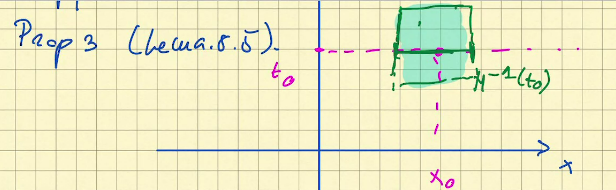
\includegraphics[scale=.5]{Visan-Lemma-8.3}
    \caption{Property 1 (Lemma 8.3 in Visan)}
    \label{fig:lem8.3}
  \end{figure}

  And then says that space-time norm of the solution is concentrated in adjacent
  rectangles?
  \begin{center}
    \begin{figure}[H]
      \centering 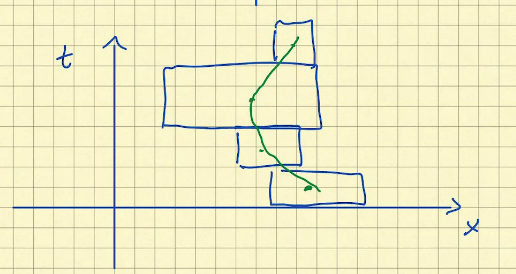
\includegraphics[scale=.5]{Visan-Lemma-8.4}
      \caption{Property 1 (Corollary 8.4 in Visan ?)}
      \label{fig:lem8.4}
    \end{figure}
  \end{center}
  
  \item \textbf{Property 2 (Corollary 8.4[V])} This property is about the
  behavior of the frequency-scale function $N$. As $t\to\infty$,
  $N(t)\to \infty$. \pnote{(Is this it?)}

  

 
  \begin{figure}[H]
    \centering 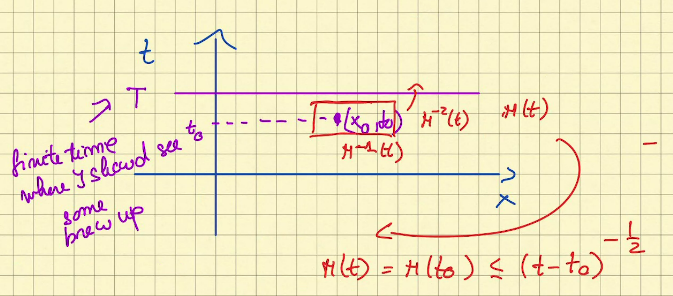
\includegraphics[scale=.6]{Visan-Lemma-8.5}
    \caption{Property 2 (Lemma 8.4 in Visan)}
    \label{fig:lem8.5}
  \end{figure}
\end{itemize}

\begin{figure}[H]
  \centering
  \includegraphics[scale=.5,trim={0 12.1cm 2cm 0},clip]{Duhamel-Reduced}
  \caption{Lemma 8.4[V]}
  \label{fig:lem8.4}
\end{figure}

\textbf{Property 3 (Lemma 8.5[V])} which says that the Strichartz norms
of the solution $u$ satisfies
\begin{equation*}
  \int_{I}N(t)^{2} dt  \lesssim \norm{u}_{L_{t,x}^{\frac{2(d+2)}{d-2}}} \leq 1 +\int_{I} N(t)^{2}dt 
\end{equation*}


Then \textbf{Lemma 8.6[V]} will give a similar bound
\begin{equation*}
  \norm{\nabla u}_{L_{t}^{2}L_{x}^{\frac{2d}{d-2}}} \lesssim 1 + \int_{I}N(t)^{2}dt 
\end{equation*}

and then \textbf{Proposition 8.7[V] (Duhamel Reduced)} says that that for the minimal
blowup solution, the portion of the $u$ which is not the Duhamel term converges
weakly to zero in $\mathring{H}_{x}^{1}$. That is, as $t_{2}\to 0,$

\begin{equation*}
  u(t_{1}) 
  = \underbrace{e^{(t_{1}-t_{2})}u(t_{2})}_{\to 0 \text{ weakly}} +
    \underbrace{\int_{t_{1}}^{t_{2}}e^{i(t_{1}-t_{2})\Delta }|u|^{2}u
    dt_{1}}_{\text{Duhamel Term}}
\end{equation*}

\pnote{Is this right?}
This is essential for proving long-time Strichartz, but not used elsewhere.



\subsection{Closing the Argument}
Now, let's eliminate the existence of such a minimal blow-up solution. First, we
get either (A) that
\begin{equation*}
  \int_{0}^{T_{\rm max}}N(t)^{-1} dt <8 
\end{equation*}
(by putting all the lemmas together), or you get (B) that
\begin{equation}\label{eq:19-caseb}
  \int_{0}^{T_{\rm max}} N(t)^{-1}dt = \infty.
\end{equation}
To preclude case (A), we use a long-time Strichartz estimate from Dodson. To
preclude case (B), we use something called the ``Interaction Morawetz
estimate''.

\subsection{Case (A): Discussion of the Long-Time Strichartz Estimate}

The Long-Strichartz Estimate is \textbf{Theorem 9.1[V]}.

Let $u: [0,T_{\rm max}]\times \R^{4}\to \mathbb{C}$, with $N(t) \equiv N_{k}
\geq 1$ on each subinterval $J_{k}$ of $[0,T_{\rm max})$. Then for each compact
time interval $I\subset [0,T_{\rm max})$ (think: $I=J_{1}\sqcup J_{2}\sqcup
\cdots \sqcup J_{k}$), we have
\begin{equation*}
  \norm{\nabla u_{ \leq  m}}_{L_{t}^{2}L_{x}^{4}(I\times \R^4)}\lesssim1 + m^{3/2}k^{1/2}
\end{equation*}
for energy $m>0$, where $k = \int_{I} N(t)^{-1}dt<\infty$.

We won't go through the proof in class, but it's not bad -- it uses standard
inequalities, Bernstein, etc. And then this long Strichartz estimate will be
used in the ``no rapid frequency cascade'' theorem which will show that the mass
$M(t)\equiv 0$ but this is a contradiction because $u$ is not identically zero.
These are the main ideas of the proof.

\subsection{Case (B): Discussion of the Interaction Morawetz Estimate}
Here we will discuss why \cref{eq:19-caseb} can't happen. Why? First, consider
the following easy case where we assume the solution is radially symmetric (this
assumption is not made for the general proof, but we are using it to illustrate
the main idea).  Introduce a functional called the \textbf{Morawetz action}:
\begin{equation*}
  M(t) := 2 \mathrm{Im} \int_{\R^{4}}\overline{u(t,x)}\nabla u(t,x) \cdot \frac{x}{|x|}dx
\end{equation*}
imagine $u$ is a solution to energy critical NLS (defocusing) made of many
particles and centered around $x$. We have

\begin{equation*}
  \partial_{t}M(t) 
  \geq 2 \int_{\R^{4}} \frac{\left| u(t,x) \right|^{2}}{|x|^{3}}dx
  + \int_{\R^{4}} \frac{\left| u(t,x) \right|^{4}}{|x|}dx  
\end{equation*}
Then integrating with respect to time and using the Cauchy-Schwarz inequality, 
\begin{equation*}
  \int_{I}\int_{\R^{4}} \frac{\left| u(t,x) \right|^{4}}{|x|}dxdt 
  \leq \norm{u}_{L^{\infty}_{t}L_{x}^{2}(I \times \R^{4})} \norm{u}_{L^{\infty}_{t}\mathring{H}_{x}^{1}}
\end{equation*}
So we have $u\in H_{x}^{1}$ (because $u\in L^{2}$ and its gradient is in
$\mathring{H}^{1}$). But this raises an issue: (1) it favors the origin and (2)
it says that $u\in H_{x}^{1}$, but our solution $u$ was constructed
as a limit of $\mathring{H}_{x}^{1}$ functions.

A modification can be shown:
\begin{equation*}
  \int_{I}\int_{|x| \leq A |I|^{\frac{1}{2}}} \frac{\left| u(t,x) \right|^{4}}{|x|}dxdt 
  \lesssim A|I|^{\frac{1}{2}} \norm{u}_{L_{t}^{\infty}\mathring{H}_{x}^{1}(I\times \R^{4})}^{2}
\end{equation*}
and we can use this now Morawetz estimate to preclude case (B).

\textbf{Step 1.} We claim that the $u(t)$ that we got from Therem 8.1[V], plus
the additional assumption of radial symmetry, is concentrated near the origin.
To prove this, consider if there is concentration of energy at a point away from
the origin (i.e. at some point with $|x| \geq N(t)^{-1}$), then by radial
symmetry the energy is concentrated at other points too, as shown in
\cref{fig:radial-symmetry}. So only concentration at the origin is possible.

\begin{figure}[h]
  \centering
  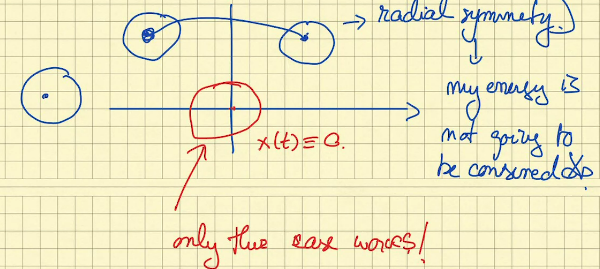
\includegraphics[scale=.5]{radial-symmetry}
  \caption{Step 1.}
  \label{fig:radial-symmetry}
\end{figure}


\textbf{Step 2.} Skipping some steps we get the following inequality which
precludes case (B):
\begin{equation*}
  |I|^{\frac{1}{2}} \geq  \int_{I} N(t)dt.
\end{equation*}


So far we have assumed radial symmetry to preclude case (B). But we can do a similar arugment without
that assupmtion. For the general case, we substitute the Morawetz inequality by
the \textbf{interaction Morawetz inequality}:
\begin{equation*}
  M_{\rm interaction}(t) 
  = 2 \mathrm{Im} \int_{\R^4 }\int_{\R^4 }  \overline{u(t,x)}\nabla u(t,x) \frac{x-y}{|x-y|} \left| u(t,y) \right|^{2}dxdy
\end{equation*}
which is the version that is frequency-localized. We have outlined the main
ideas. Next time we will go through how to do global existence for things that
look like NLS: i.e. which linearly look like NLS and are defocusing. We will be
able to eliminate some assumptions (e.g. localization and some conservation
quantities). We will get some global-in-time Strichartz.

\section{Lecture: 2022-12-06}
Topic: Local well-posedness for the defocusing Model NLS (MNLS), which is
\begin{equation*}
  \left\{ \begin{array}{l@{}l}
      iu_{t}+u_{xx}=C(u,\bar{u},u) \\
      u(0,x)=u_{0}
    \end{array}\right.
\end{equation*}
Here, $X \subset C([0,1],L^{2})$.  First use a fixed point argument to get LWP
(using $X$, Duhamel formula). Then you can go further for global.

This is \textbf{Prop 1.38[Tao]} which splits the fixed point argument into two bits: a
linear and nonlinear part, which are treated differently. Two estimates:
\begin{itemize}
  \item (Linear Part). The space $X$ has norm
  \begin{equation*}
    \norm{u}_{X}^{2} = \sum_{k\in \mathbb{Z}}  \norm{u_{k}}_{X_{k}}
  \end{equation*}
  where
  \begin{equation*}
    \norm{u_{k}}_{X_{k}}= \sum_{j\in \mathbb{Z}}
    \norm{\chi_{j}(t,x-2tk)u_{k}}_{L_{t}^{\infty}L_{x}^{2}}^{2}
  \end{equation*}
  where $\left\{\chi_{k}: k\in \mathbb{Z}\right\}$ is a partition of unity in
  \textit{space} (i.e. the $x$ variable). So now we also need the $Y$ and we
  choose it so that its dual is $X$, i.e. $Y^{*} = X$. Then
  \begin{equation*}
    \norm{f}_{Y}^{2} = \sum_{k\in \mathbb{Z}}\norm{f_{k}}_{Y_{k}}^{2} 
  \end{equation*}
  where
  \begin{equation*}
    \norm{f_{k}}_{Y_{k}}^{2} = \sum_{j\in \mathbb{Z}}\norm{\lambda_{j}(t,x-2kt)f_{k}}_{L_{t}^{1}L_{x}^{2}}^{2}
  \end{equation*}
  \textbf{Lemma 3.3} gives the solution to the linear Schroedinger equation
  \begin{equation*}
    \left\{ \begin{array}{l@{}l}
        (iu_{t}+\partial_{x}^{2})u= f\\
        u(0,x)=u_{0}
      \end{array}\right.
  \end{equation*}
  in the time interval $[0,1]$ satisfies
  \begin{equation}\label{eq:19}
    \norm{u}_{X} \lesssim \norm{u_{0}}_{L^{2}}+ \norm{f}_{Y}
  \end{equation}
  \item (Nonlinear Part). By \textbf{Lemma 3.4} for the cubic nonlinearity $C$,
  we have the bound 
  \begin{equation}\label{eq:20}
    \norm{C(u,\bar{u},u)}_{Y}\lesssim \norm{u}_{X}^{3}
  \end{equation}
      
\end{itemize}
Then using the estimates for these two cases, we obtain a contraction and apply
the fixed point theorem. First we will prove \textbf{Lemma 3.3}:

\begin{proof}[Proof of \cref{eq:19}]
  It suffices to prove
  \begin{equation}\label{eq:21}
    \norm{u_{k}}_{X_{k}} \lesssim \norm{u_{0,k}}_{L^{2}} +\norm{f_{k}}_{X_{k}}
  \end{equation}
  because we can then sum over $k$ which then gives \cref{eq:19}. Using
  Galileian invariance to move from frequency $k$ to frequency $0$. Define
  \begin{equation*}
    v(t,x) = e^{-i(kx+k^{2}t)}u_{k}(t,x-2kt)
  \end{equation*}
  and
  \begin{equation*}
    v_{0}(0,x) = e^{-ikx}u_{0,k}
  \end{equation*}
  and
  \begin{equation*}
    g(t,x) = e^{-i(kx+k^{2}t)}f_{k}(t,x=2kt).
  \end{equation*}
  Observe that $v,v_{0},$ and $g$ satisfy
  \begin{equation*}
    (i\partial_{t}+\partial_{x})v = g \quad \text{ with}\quad v(0)=v_{0}
  \end{equation*}
  Then we claim that \cref{eq:21} transforms to
  \begin{equation}\label{eq:22}
    \norm{v}_{X_{0}} \lesssim \norm{v_{0}}_{L^{2}}+\norm{g}_{Y_{0}}
  \end{equation}
  How do we prove \cref{eq:22}? By Duhamel,
  \begin{equation*}
    v(t) 
    = e^{it\partial_{x}^{2}}P_{0}v_{0}
    + \int_{0}^{t}e^{i(t-s)\partial_{x}^{2}}P_{0}gds 
  \end{equation*}
  where $P_{0}$ is a projection. Now we need to localize $v(t)$ spatially:
  \begin{equation}\label{eq:23}
    \chi_{j}v(t) 
    = \sum_{\ell\in\mathbb{Z}}\left(\chi_{j}e^{it\partial_{x}^{2}}
      P_{0}\chi_{\ell}\ v_{0}
      +\int_{0}^{t}\chi_{j}e^{i(t-s)\partial_{x}^{2}}
      P_{0}\chi_{\ell}\ g ds  \right)  
  \end{equation}
  The $\chi_{\ell}$ is necessary to measure the intial data and source term in
  $X_{0}$. Observe that the kernels $e^{it\partial_{x}^{2}}P_{0}$ are uniformly
  Schwarz on $[0,1]$. So one has $L^{2}$ bound with off-diagonal decay:
  \begin{equation*}
    \norm{\chi_{j}e^{it\partial_{x}^{2}}P_{0}\chi_{\ell}}_{L^2\to L^2}
    \lesssim
    \left\langle j-\ell \right\rangle^{-N}
  \end{equation*}
  where the right-hand side uses the Japanese bracket. This estimate is why we
  needed the $P_{0}$, because otherwise we wouldn't have this. Now we take
  \cref{eq:23} and
  \begin{equation*}
    \norm{\chi_{j}v}_{L_{t}^{\infty}L_{x}^{2}} \lesssim \sum_{\ell\in \mathbb{Z}} \left\langle j-\ell \right\rangle^{-N}\left( \norm{\chi_{\ell}v_{0}}_{L_{x}^{2}}+\norm{\chi_{\ell}g}_{L_{t}^{1}L_{x}^{2}} \right). 
  \end{equation*}
\end{proof}
Next we will discuss \textbf{Lemma 3.4}. We will actually need a stronger
estimate which is specific to the frequency. We first need to define
\textbf{frequency envelopes}.
\begin{definition}[Frequency Envelope]
  \label{def:frequency-envelope}
  Let $\left\{c_{k}\right\}_{k}\subset \ell^{2}$. We say that
  $\left\{c_{k}\right\}$ is a \textbf{frequency envelope} for $u_{0}$ in $L^2$
  if
  \begin{enumerate}
    \item $\norm{P_{k}u_{0}}_{L^2} \leq c_{k}$
    \item $c_{k}$ is \textit{slowly varying} in that $\frac{c_{j}}{c_{k}}\leq 2^{\delta \left| j-k \right|}$. (This is a picture).
  \end{enumerate}
\end{definition}
We will modify this definition for our setting using a maximal function. A
rigorous modification of this definition will be provided in the next class.
Then we will prove \textbf{lemma 3.4} with and without frequency envelopes. 
\end{document}

\bibliographystyle{siam.bst}
\bibliography{bibliography}
